% Created by tikzDevice version 0.12.3 on 2020-04-04 19:24:30
% !TEX encoding = UTF-8 Unicode
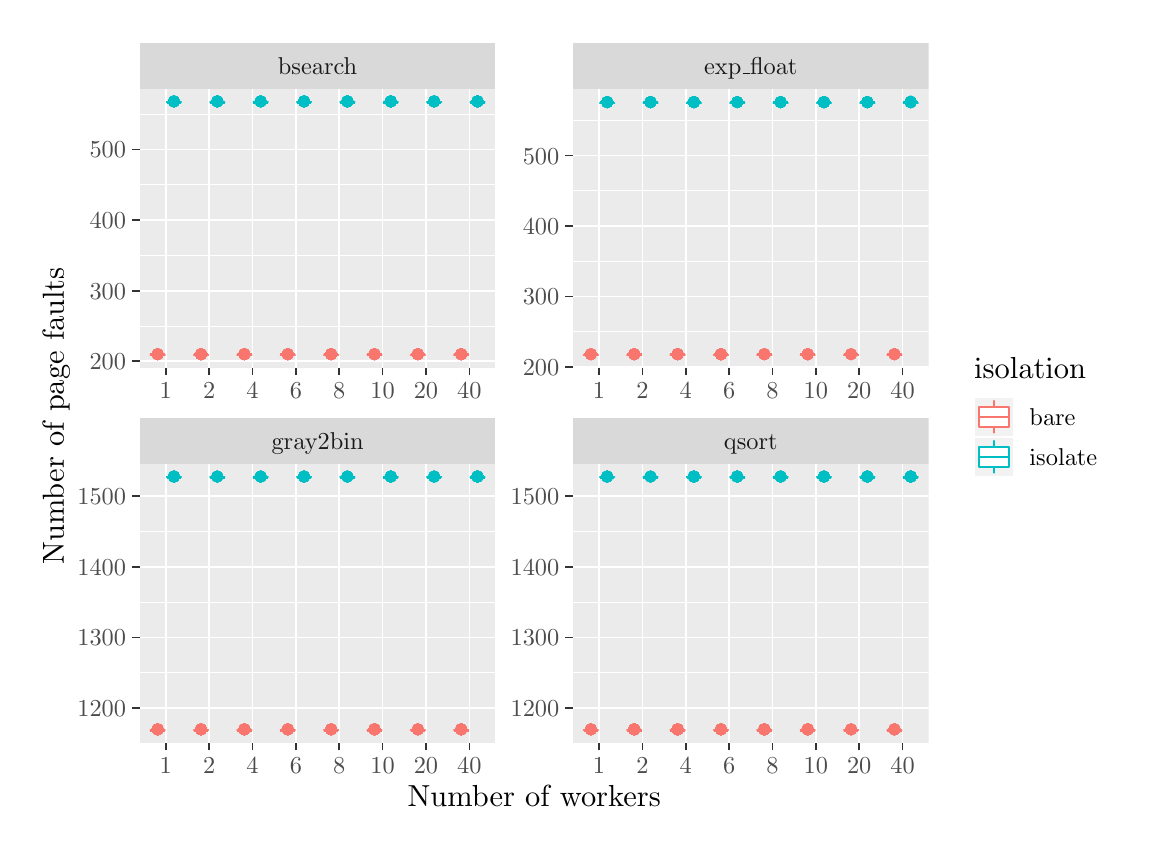
\begin{tikzpicture}[x=1pt,y=1pt]
\definecolor{fillColor}{RGB}{255,255,255}
\path[use as bounding box,fill=fillColor,fill opacity=0.00] (0,0) rectangle (397.48,289.08);
\begin{scope}
\path[clip] (  0.00,  0.00) rectangle (397.48,289.08);
\definecolor{drawColor}{RGB}{255,255,255}
\definecolor{fillColor}{RGB}{255,255,255}

\path[draw=drawColor,line width= 0.6pt,line join=round,line cap=round,fill=fillColor] (  0.00,  0.00) rectangle (397.48,289.08);
\end{scope}
\begin{scope}
\path[clip] ( 40.51,166.24) rectangle (169.00,267.01);
\definecolor{fillColor}{gray}{0.92}

\path[fill=fillColor] ( 40.51,166.24) rectangle (169.00,267.01);
\definecolor{drawColor}{RGB}{255,255,255}

\path[draw=drawColor,line width= 0.3pt,line join=round] ( 40.51,181.29) --
	(169.00,181.29);

\path[draw=drawColor,line width= 0.3pt,line join=round] ( 40.51,206.80) --
	(169.00,206.80);

\path[draw=drawColor,line width= 0.3pt,line join=round] ( 40.51,232.32) --
	(169.00,232.32);

\path[draw=drawColor,line width= 0.3pt,line join=round] ( 40.51,257.84) --
	(169.00,257.84);

\path[draw=drawColor,line width= 0.6pt,line join=round] ( 40.51,168.53) --
	(169.00,168.53);

\path[draw=drawColor,line width= 0.6pt,line join=round] ( 40.51,194.04) --
	(169.00,194.04);

\path[draw=drawColor,line width= 0.6pt,line join=round] ( 40.51,219.56) --
	(169.00,219.56);

\path[draw=drawColor,line width= 0.6pt,line join=round] ( 40.51,245.08) --
	(169.00,245.08);

\path[draw=drawColor,line width= 0.6pt,line join=round] ( 49.91,166.24) --
	( 49.91,267.01);

\path[draw=drawColor,line width= 0.6pt,line join=round] ( 65.58,166.24) --
	( 65.58,267.01);

\path[draw=drawColor,line width= 0.6pt,line join=round] ( 81.25,166.24) --
	( 81.25,267.01);

\path[draw=drawColor,line width= 0.6pt,line join=round] ( 96.92,166.24) --
	( 96.92,267.01);

\path[draw=drawColor,line width= 0.6pt,line join=round] (112.59,166.24) --
	(112.59,267.01);

\path[draw=drawColor,line width= 0.6pt,line join=round] (128.26,166.24) --
	(128.26,267.01);

\path[draw=drawColor,line width= 0.6pt,line join=round] (143.93,166.24) --
	(143.93,267.01);

\path[draw=drawColor,line width= 0.6pt,line join=round] (159.60,166.24) --
	(159.60,267.01);
\definecolor{drawColor}{RGB}{248,118,109}
\definecolor{fillColor}{RGB}{248,118,109}

\path[draw=drawColor,line width= 0.4pt,line join=round,line cap=round,fill=fillColor] ( 46.97,171.08) circle (  1.96);

\path[draw=drawColor,line width= 0.4pt,line join=round,line cap=round,fill=fillColor] ( 46.97,171.08) circle (  1.96);

\path[draw=drawColor,line width= 0.4pt,line join=round,line cap=round,fill=fillColor] ( 46.97,171.08) circle (  1.96);

\path[draw=drawColor,line width= 0.4pt,line join=round,line cap=round,fill=fillColor] ( 46.97,171.08) circle (  1.96);

\path[draw=drawColor,line width= 0.4pt,line join=round,line cap=round,fill=fillColor] ( 46.97,171.08) circle (  1.96);

\path[draw=drawColor,line width= 0.4pt,line join=round,line cap=round,fill=fillColor] ( 46.97,171.08) circle (  1.96);

\path[draw=drawColor,line width= 0.4pt,line join=round,line cap=round,fill=fillColor] ( 46.97,171.08) circle (  1.96);

\path[draw=drawColor,line width= 0.4pt,line join=round,line cap=round,fill=fillColor] ( 46.97,171.08) circle (  1.96);

\path[draw=drawColor,line width= 0.6pt,line join=round] ( 46.97,170.82) -- ( 46.97,170.82);

\path[draw=drawColor,line width= 0.6pt,line join=round] ( 46.97,170.82) -- ( 46.97,170.82);
\definecolor{fillColor}{RGB}{255,255,255}

\path[draw=drawColor,line width= 0.6pt,line join=round,line cap=round,fill=fillColor] ( 44.33,170.82) --
	( 44.33,170.82) --
	( 49.62,170.82) --
	( 49.62,170.82) --
	( 44.33,170.82) --
	cycle;

\path[draw=drawColor,line width= 1.1pt,line join=round] ( 44.33,170.82) -- ( 49.62,170.82);
\definecolor{drawColor}{RGB}{0,191,196}
\definecolor{fillColor}{RGB}{0,191,196}

\path[draw=drawColor,line width= 0.4pt,line join=round,line cap=round,fill=fillColor] ( 52.85,262.43) circle (  1.96);

\path[draw=drawColor,line width= 0.4pt,line join=round,line cap=round,fill=fillColor] ( 52.85,262.43) circle (  1.96);

\path[draw=drawColor,line width= 0.4pt,line join=round,line cap=round,fill=fillColor] ( 52.85,262.43) circle (  1.96);

\path[draw=drawColor,line width= 0.4pt,line join=round,line cap=round,fill=fillColor] ( 52.85,262.43) circle (  1.96);

\path[draw=drawColor,line width= 0.4pt,line join=round,line cap=round,fill=fillColor] ( 52.85,262.43) circle (  1.96);

\path[draw=drawColor,line width= 0.4pt,line join=round,line cap=round,fill=fillColor] ( 52.85,262.43) circle (  1.96);

\path[draw=drawColor,line width= 0.4pt,line join=round,line cap=round,fill=fillColor] ( 52.85,262.43) circle (  1.96);

\path[draw=drawColor,line width= 0.4pt,line join=round,line cap=round,fill=fillColor] ( 52.85,262.43) circle (  1.96);

\path[draw=drawColor,line width= 0.4pt,line join=round,line cap=round,fill=fillColor] ( 52.85,262.43) circle (  1.96);

\path[draw=drawColor,line width= 0.6pt,line join=round] ( 52.85,262.17) -- ( 52.85,262.17);

\path[draw=drawColor,line width= 0.6pt,line join=round] ( 52.85,262.17) -- ( 52.85,262.17);
\definecolor{fillColor}{RGB}{255,255,255}

\path[draw=drawColor,line width= 0.6pt,line join=round,line cap=round,fill=fillColor] ( 50.21,262.17) --
	( 50.21,262.17) --
	( 55.49,262.17) --
	( 55.49,262.17) --
	( 50.21,262.17) --
	cycle;

\path[draw=drawColor,line width= 1.1pt,line join=round] ( 50.21,262.17) -- ( 55.49,262.17);
\definecolor{drawColor}{RGB}{248,118,109}
\definecolor{fillColor}{RGB}{248,118,109}

\path[draw=drawColor,line width= 0.4pt,line join=round,line cap=round,fill=fillColor] ( 62.64,171.08) circle (  1.96);

\path[draw=drawColor,line width= 0.4pt,line join=round,line cap=round,fill=fillColor] ( 62.64,171.08) circle (  1.96);

\path[draw=drawColor,line width= 0.4pt,line join=round,line cap=round,fill=fillColor] ( 62.64,171.08) circle (  1.96);

\path[draw=drawColor,line width= 0.4pt,line join=round,line cap=round,fill=fillColor] ( 62.64,171.08) circle (  1.96);

\path[draw=drawColor,line width= 0.4pt,line join=round,line cap=round,fill=fillColor] ( 62.64,171.08) circle (  1.96);

\path[draw=drawColor,line width= 0.4pt,line join=round,line cap=round,fill=fillColor] ( 62.64,171.08) circle (  1.96);

\path[draw=drawColor,line width= 0.4pt,line join=round,line cap=round,fill=fillColor] ( 62.64,171.08) circle (  1.96);

\path[draw=drawColor,line width= 0.4pt,line join=round,line cap=round,fill=fillColor] ( 62.64,171.08) circle (  1.96);

\path[draw=drawColor,line width= 0.4pt,line join=round,line cap=round,fill=fillColor] ( 62.64,171.08) circle (  1.96);

\path[draw=drawColor,line width= 0.4pt,line join=round,line cap=round,fill=fillColor] ( 62.64,171.08) circle (  1.96);

\path[draw=drawColor,line width= 0.4pt,line join=round,line cap=round,fill=fillColor] ( 62.64,171.08) circle (  1.96);

\path[draw=drawColor,line width= 0.4pt,line join=round,line cap=round,fill=fillColor] ( 62.64,171.08) circle (  1.96);

\path[draw=drawColor,line width= 0.4pt,line join=round,line cap=round,fill=fillColor] ( 62.64,171.08) circle (  1.96);

\path[draw=drawColor,line width= 0.6pt,line join=round] ( 62.64,170.82) -- ( 62.64,170.82);

\path[draw=drawColor,line width= 0.6pt,line join=round] ( 62.64,170.82) -- ( 62.64,170.82);
\definecolor{fillColor}{RGB}{255,255,255}

\path[draw=drawColor,line width= 0.6pt,line join=round,line cap=round,fill=fillColor] ( 60.00,170.82) --
	( 60.00,170.82) --
	( 65.29,170.82) --
	( 65.29,170.82) --
	( 60.00,170.82) --
	cycle;

\path[draw=drawColor,line width= 1.1pt,line join=round] ( 60.00,170.82) -- ( 65.29,170.82);
\definecolor{drawColor}{RGB}{0,191,196}
\definecolor{fillColor}{RGB}{0,191,196}

\path[draw=drawColor,line width= 0.4pt,line join=round,line cap=round,fill=fillColor] ( 68.52,262.43) circle (  1.96);

\path[draw=drawColor,line width= 0.4pt,line join=round,line cap=round,fill=fillColor] ( 68.52,262.43) circle (  1.96);

\path[draw=drawColor,line width= 0.4pt,line join=round,line cap=round,fill=fillColor] ( 68.52,262.43) circle (  1.96);

\path[draw=drawColor,line width= 0.4pt,line join=round,line cap=round,fill=fillColor] ( 68.52,262.43) circle (  1.96);

\path[draw=drawColor,line width= 0.4pt,line join=round,line cap=round,fill=fillColor] ( 68.52,262.43) circle (  1.96);

\path[draw=drawColor,line width= 0.4pt,line join=round,line cap=round,fill=fillColor] ( 68.52,262.43) circle (  1.96);

\path[draw=drawColor,line width= 0.4pt,line join=round,line cap=round,fill=fillColor] ( 68.52,262.43) circle (  1.96);

\path[draw=drawColor,line width= 0.4pt,line join=round,line cap=round,fill=fillColor] ( 68.52,262.43) circle (  1.96);

\path[draw=drawColor,line width= 0.4pt,line join=round,line cap=round,fill=fillColor] ( 68.52,262.43) circle (  1.96);

\path[draw=drawColor,line width= 0.6pt,line join=round] ( 68.52,262.17) -- ( 68.52,262.17);

\path[draw=drawColor,line width= 0.6pt,line join=round] ( 68.52,262.17) -- ( 68.52,262.17);
\definecolor{fillColor}{RGB}{255,255,255}

\path[draw=drawColor,line width= 0.6pt,line join=round,line cap=round,fill=fillColor] ( 65.88,262.17) --
	( 65.88,262.17) --
	( 71.16,262.17) --
	( 71.16,262.17) --
	( 65.88,262.17) --
	cycle;

\path[draw=drawColor,line width= 1.1pt,line join=round] ( 65.88,262.17) -- ( 71.16,262.17);
\definecolor{drawColor}{RGB}{248,118,109}
\definecolor{fillColor}{RGB}{248,118,109}

\path[draw=drawColor,line width= 0.4pt,line join=round,line cap=round,fill=fillColor] ( 78.31,171.08) circle (  1.96);

\path[draw=drawColor,line width= 0.4pt,line join=round,line cap=round,fill=fillColor] ( 78.31,171.08) circle (  1.96);

\path[draw=drawColor,line width= 0.4pt,line join=round,line cap=round,fill=fillColor] ( 78.31,171.08) circle (  1.96);

\path[draw=drawColor,line width= 0.4pt,line join=round,line cap=round,fill=fillColor] ( 78.31,171.08) circle (  1.96);

\path[draw=drawColor,line width= 0.4pt,line join=round,line cap=round,fill=fillColor] ( 78.31,171.08) circle (  1.96);

\path[draw=drawColor,line width= 0.4pt,line join=round,line cap=round,fill=fillColor] ( 78.31,171.08) circle (  1.96);

\path[draw=drawColor,line width= 0.4pt,line join=round,line cap=round,fill=fillColor] ( 78.31,171.08) circle (  1.96);

\path[draw=drawColor,line width= 0.4pt,line join=round,line cap=round,fill=fillColor] ( 78.31,171.08) circle (  1.96);

\path[draw=drawColor,line width= 0.4pt,line join=round,line cap=round,fill=fillColor] ( 78.31,171.08) circle (  1.96);

\path[draw=drawColor,line width= 0.4pt,line join=round,line cap=round,fill=fillColor] ( 78.31,171.08) circle (  1.96);

\path[draw=drawColor,line width= 0.6pt,line join=round] ( 78.31,170.82) -- ( 78.31,170.82);

\path[draw=drawColor,line width= 0.6pt,line join=round] ( 78.31,170.82) -- ( 78.31,170.82);
\definecolor{fillColor}{RGB}{255,255,255}

\path[draw=drawColor,line width= 0.6pt,line join=round,line cap=round,fill=fillColor] ( 75.67,170.82) --
	( 75.67,170.82) --
	( 80.96,170.82) --
	( 80.96,170.82) --
	( 75.67,170.82) --
	cycle;

\path[draw=drawColor,line width= 1.1pt,line join=round] ( 75.67,170.82) -- ( 80.96,170.82);
\definecolor{drawColor}{RGB}{0,191,196}
\definecolor{fillColor}{RGB}{0,191,196}

\path[draw=drawColor,line width= 0.4pt,line join=round,line cap=round,fill=fillColor] ( 84.19,262.43) circle (  1.96);

\path[draw=drawColor,line width= 0.4pt,line join=round,line cap=round,fill=fillColor] ( 84.19,262.43) circle (  1.96);

\path[draw=drawColor,line width= 0.4pt,line join=round,line cap=round,fill=fillColor] ( 84.19,262.43) circle (  1.96);

\path[draw=drawColor,line width= 0.4pt,line join=round,line cap=round,fill=fillColor] ( 84.19,262.43) circle (  1.96);

\path[draw=drawColor,line width= 0.4pt,line join=round,line cap=round,fill=fillColor] ( 84.19,262.43) circle (  1.96);

\path[draw=drawColor,line width= 0.4pt,line join=round,line cap=round,fill=fillColor] ( 84.19,262.43) circle (  1.96);

\path[draw=drawColor,line width= 0.4pt,line join=round,line cap=round,fill=fillColor] ( 84.19,262.43) circle (  1.96);

\path[draw=drawColor,line width= 0.4pt,line join=round,line cap=round,fill=fillColor] ( 84.19,262.43) circle (  1.96);

\path[draw=drawColor,line width= 0.6pt,line join=round] ( 84.19,262.17) -- ( 84.19,262.17);

\path[draw=drawColor,line width= 0.6pt,line join=round] ( 84.19,262.17) -- ( 84.19,262.17);
\definecolor{fillColor}{RGB}{255,255,255}

\path[draw=drawColor,line width= 0.6pt,line join=round,line cap=round,fill=fillColor] ( 81.55,262.17) --
	( 81.55,262.17) --
	( 86.83,262.17) --
	( 86.83,262.17) --
	( 81.55,262.17) --
	cycle;

\path[draw=drawColor,line width= 1.1pt,line join=round] ( 81.55,262.17) -- ( 86.83,262.17);
\definecolor{drawColor}{RGB}{248,118,109}
\definecolor{fillColor}{RGB}{248,118,109}

\path[draw=drawColor,line width= 0.4pt,line join=round,line cap=round,fill=fillColor] ( 93.98,171.08) circle (  1.96);

\path[draw=drawColor,line width= 0.4pt,line join=round,line cap=round,fill=fillColor] ( 93.98,171.08) circle (  1.96);

\path[draw=drawColor,line width= 0.4pt,line join=round,line cap=round,fill=fillColor] ( 93.98,171.08) circle (  1.96);

\path[draw=drawColor,line width= 0.4pt,line join=round,line cap=round,fill=fillColor] ( 93.98,171.08) circle (  1.96);

\path[draw=drawColor,line width= 0.4pt,line join=round,line cap=round,fill=fillColor] ( 93.98,171.08) circle (  1.96);

\path[draw=drawColor,line width= 0.4pt,line join=round,line cap=round,fill=fillColor] ( 93.98,171.08) circle (  1.96);

\path[draw=drawColor,line width= 0.4pt,line join=round,line cap=round,fill=fillColor] ( 93.98,171.08) circle (  1.96);

\path[draw=drawColor,line width= 0.4pt,line join=round,line cap=round,fill=fillColor] ( 93.98,171.08) circle (  1.96);

\path[draw=drawColor,line width= 0.4pt,line join=round,line cap=round,fill=fillColor] ( 93.98,171.08) circle (  1.96);

\path[draw=drawColor,line width= 0.4pt,line join=round,line cap=round,fill=fillColor] ( 93.98,171.08) circle (  1.96);

\path[draw=drawColor,line width= 0.6pt,line join=round] ( 93.98,170.82) -- ( 93.98,170.82);

\path[draw=drawColor,line width= 0.6pt,line join=round] ( 93.98,170.82) -- ( 93.98,170.82);
\definecolor{fillColor}{RGB}{255,255,255}

\path[draw=drawColor,line width= 0.6pt,line join=round,line cap=round,fill=fillColor] ( 91.34,170.82) --
	( 91.34,170.82) --
	( 96.63,170.82) --
	( 96.63,170.82) --
	( 91.34,170.82) --
	cycle;

\path[draw=drawColor,line width= 1.1pt,line join=round] ( 91.34,170.82) -- ( 96.63,170.82);
\definecolor{drawColor}{RGB}{0,191,196}
\definecolor{fillColor}{RGB}{0,191,196}

\path[draw=drawColor,line width= 0.4pt,line join=round,line cap=round,fill=fillColor] ( 99.86,262.43) circle (  1.96);

\path[draw=drawColor,line width= 0.4pt,line join=round,line cap=round,fill=fillColor] ( 99.86,262.43) circle (  1.96);

\path[draw=drawColor,line width= 0.4pt,line join=round,line cap=round,fill=fillColor] ( 99.86,262.43) circle (  1.96);

\path[draw=drawColor,line width= 0.4pt,line join=round,line cap=round,fill=fillColor] ( 99.86,262.43) circle (  1.96);

\path[draw=drawColor,line width= 0.4pt,line join=round,line cap=round,fill=fillColor] ( 99.86,262.43) circle (  1.96);

\path[draw=drawColor,line width= 0.4pt,line join=round,line cap=round,fill=fillColor] ( 99.86,262.43) circle (  1.96);

\path[draw=drawColor,line width= 0.4pt,line join=round,line cap=round,fill=fillColor] ( 99.86,262.43) circle (  1.96);

\path[draw=drawColor,line width= 0.4pt,line join=round,line cap=round,fill=fillColor] ( 99.86,262.43) circle (  1.96);

\path[draw=drawColor,line width= 0.4pt,line join=round,line cap=round,fill=fillColor] ( 99.86,262.43) circle (  1.96);

\path[draw=drawColor,line width= 0.4pt,line join=round,line cap=round,fill=fillColor] ( 99.86,262.43) circle (  1.96);

\path[draw=drawColor,line width= 0.6pt,line join=round] ( 99.86,262.17) -- ( 99.86,262.17);

\path[draw=drawColor,line width= 0.6pt,line join=round] ( 99.86,262.17) -- ( 99.86,262.17);
\definecolor{fillColor}{RGB}{255,255,255}

\path[draw=drawColor,line width= 0.6pt,line join=round,line cap=round,fill=fillColor] ( 97.22,262.17) --
	( 97.22,262.17) --
	(102.50,262.17) --
	(102.50,262.17) --
	( 97.22,262.17) --
	cycle;

\path[draw=drawColor,line width= 1.1pt,line join=round] ( 97.22,262.17) -- (102.50,262.17);
\definecolor{drawColor}{RGB}{248,118,109}
\definecolor{fillColor}{RGB}{248,118,109}

\path[draw=drawColor,line width= 0.4pt,line join=round,line cap=round,fill=fillColor] (109.65,171.08) circle (  1.96);

\path[draw=drawColor,line width= 0.4pt,line join=round,line cap=round,fill=fillColor] (109.65,171.08) circle (  1.96);

\path[draw=drawColor,line width= 0.4pt,line join=round,line cap=round,fill=fillColor] (109.65,171.08) circle (  1.96);

\path[draw=drawColor,line width= 0.4pt,line join=round,line cap=round,fill=fillColor] (109.65,171.08) circle (  1.96);

\path[draw=drawColor,line width= 0.4pt,line join=round,line cap=round,fill=fillColor] (109.65,171.08) circle (  1.96);

\path[draw=drawColor,line width= 0.4pt,line join=round,line cap=round,fill=fillColor] (109.65,171.08) circle (  1.96);

\path[draw=drawColor,line width= 0.4pt,line join=round,line cap=round,fill=fillColor] (109.65,171.08) circle (  1.96);

\path[draw=drawColor,line width= 0.4pt,line join=round,line cap=round,fill=fillColor] (109.65,171.08) circle (  1.96);

\path[draw=drawColor,line width= 0.4pt,line join=round,line cap=round,fill=fillColor] (109.65,171.08) circle (  1.96);

\path[draw=drawColor,line width= 0.4pt,line join=round,line cap=round,fill=fillColor] (109.65,171.08) circle (  1.96);

\path[draw=drawColor,line width= 0.4pt,line join=round,line cap=round,fill=fillColor] (109.65,171.08) circle (  1.96);

\path[draw=drawColor,line width= 0.6pt,line join=round] (109.65,170.82) -- (109.65,170.82);

\path[draw=drawColor,line width= 0.6pt,line join=round] (109.65,170.82) -- (109.65,170.82);
\definecolor{fillColor}{RGB}{255,255,255}

\path[draw=drawColor,line width= 0.6pt,line join=round,line cap=round,fill=fillColor] (107.01,170.82) --
	(107.01,170.82) --
	(112.30,170.82) --
	(112.30,170.82) --
	(107.01,170.82) --
	cycle;

\path[draw=drawColor,line width= 1.1pt,line join=round] (107.01,170.82) -- (112.30,170.82);
\definecolor{drawColor}{RGB}{0,191,196}
\definecolor{fillColor}{RGB}{0,191,196}

\path[draw=drawColor,line width= 0.4pt,line join=round,line cap=round,fill=fillColor] (115.53,262.43) circle (  1.96);

\path[draw=drawColor,line width= 0.4pt,line join=round,line cap=round,fill=fillColor] (115.53,262.43) circle (  1.96);

\path[draw=drawColor,line width= 0.4pt,line join=round,line cap=round,fill=fillColor] (115.53,262.43) circle (  1.96);

\path[draw=drawColor,line width= 0.4pt,line join=round,line cap=round,fill=fillColor] (115.53,262.43) circle (  1.96);

\path[draw=drawColor,line width= 0.4pt,line join=round,line cap=round,fill=fillColor] (115.53,262.43) circle (  1.96);

\path[draw=drawColor,line width= 0.4pt,line join=round,line cap=round,fill=fillColor] (115.53,262.43) circle (  1.96);

\path[draw=drawColor,line width= 0.4pt,line join=round,line cap=round,fill=fillColor] (115.53,262.43) circle (  1.96);

\path[draw=drawColor,line width= 0.4pt,line join=round,line cap=round,fill=fillColor] (115.53,262.43) circle (  1.96);

\path[draw=drawColor,line width= 0.4pt,line join=round,line cap=round,fill=fillColor] (115.53,262.43) circle (  1.96);

\path[draw=drawColor,line width= 0.4pt,line join=round,line cap=round,fill=fillColor] (115.53,262.43) circle (  1.96);

\path[draw=drawColor,line width= 0.4pt,line join=round,line cap=round,fill=fillColor] (115.53,262.43) circle (  1.96);

\path[draw=drawColor,line width= 0.4pt,line join=round,line cap=round,fill=fillColor] (115.53,262.43) circle (  1.96);

\path[draw=drawColor,line width= 0.4pt,line join=round,line cap=round,fill=fillColor] (115.53,262.43) circle (  1.96);

\path[draw=drawColor,line width= 0.6pt,line join=round] (115.53,262.17) -- (115.53,262.17);

\path[draw=drawColor,line width= 0.6pt,line join=round] (115.53,262.17) -- (115.53,262.17);
\definecolor{fillColor}{RGB}{255,255,255}

\path[draw=drawColor,line width= 0.6pt,line join=round,line cap=round,fill=fillColor] (112.89,262.17) --
	(112.89,262.17) --
	(118.17,262.17) --
	(118.17,262.17) --
	(112.89,262.17) --
	cycle;

\path[draw=drawColor,line width= 1.1pt,line join=round] (112.89,262.17) -- (118.17,262.17);
\definecolor{drawColor}{RGB}{248,118,109}
\definecolor{fillColor}{RGB}{248,118,109}

\path[draw=drawColor,line width= 0.4pt,line join=round,line cap=round,fill=fillColor] (125.32,171.08) circle (  1.96);

\path[draw=drawColor,line width= 0.4pt,line join=round,line cap=round,fill=fillColor] (125.32,171.08) circle (  1.96);

\path[draw=drawColor,line width= 0.4pt,line join=round,line cap=round,fill=fillColor] (125.32,171.08) circle (  1.96);

\path[draw=drawColor,line width= 0.4pt,line join=round,line cap=round,fill=fillColor] (125.32,171.08) circle (  1.96);

\path[draw=drawColor,line width= 0.4pt,line join=round,line cap=round,fill=fillColor] (125.32,171.08) circle (  1.96);

\path[draw=drawColor,line width= 0.4pt,line join=round,line cap=round,fill=fillColor] (125.32,171.08) circle (  1.96);

\path[draw=drawColor,line width= 0.4pt,line join=round,line cap=round,fill=fillColor] (125.32,171.08) circle (  1.96);

\path[draw=drawColor,line width= 0.4pt,line join=round,line cap=round,fill=fillColor] (125.32,171.08) circle (  1.96);

\path[draw=drawColor,line width= 0.4pt,line join=round,line cap=round,fill=fillColor] (125.32,171.08) circle (  1.96);

\path[draw=drawColor,line width= 0.6pt,line join=round] (125.32,170.82) -- (125.32,170.82);

\path[draw=drawColor,line width= 0.6pt,line join=round] (125.32,170.82) -- (125.32,170.82);
\definecolor{fillColor}{RGB}{255,255,255}

\path[draw=drawColor,line width= 0.6pt,line join=round,line cap=round,fill=fillColor] (122.68,170.82) --
	(122.68,170.82) --
	(127.97,170.82) --
	(127.97,170.82) --
	(122.68,170.82) --
	cycle;

\path[draw=drawColor,line width= 1.1pt,line join=round] (122.68,170.82) -- (127.97,170.82);
\definecolor{drawColor}{RGB}{0,191,196}
\definecolor{fillColor}{RGB}{0,191,196}

\path[draw=drawColor,line width= 0.4pt,line join=round,line cap=round,fill=fillColor] (131.20,262.43) circle (  1.96);

\path[draw=drawColor,line width= 0.4pt,line join=round,line cap=round,fill=fillColor] (131.20,262.43) circle (  1.96);

\path[draw=drawColor,line width= 0.4pt,line join=round,line cap=round,fill=fillColor] (131.20,262.43) circle (  1.96);

\path[draw=drawColor,line width= 0.4pt,line join=round,line cap=round,fill=fillColor] (131.20,262.43) circle (  1.96);

\path[draw=drawColor,line width= 0.4pt,line join=round,line cap=round,fill=fillColor] (131.20,262.43) circle (  1.96);

\path[draw=drawColor,line width= 0.4pt,line join=round,line cap=round,fill=fillColor] (131.20,262.43) circle (  1.96);

\path[draw=drawColor,line width= 0.4pt,line join=round,line cap=round,fill=fillColor] (131.20,262.43) circle (  1.96);

\path[draw=drawColor,line width= 0.4pt,line join=round,line cap=round,fill=fillColor] (131.20,262.43) circle (  1.96);

\path[draw=drawColor,line width= 0.4pt,line join=round,line cap=round,fill=fillColor] (131.20,262.43) circle (  1.96);

\path[draw=drawColor,line width= 0.4pt,line join=round,line cap=round,fill=fillColor] (131.20,262.43) circle (  1.96);

\path[draw=drawColor,line width= 0.4pt,line join=round,line cap=round,fill=fillColor] (131.20,262.43) circle (  1.96);

\path[draw=drawColor,line width= 0.4pt,line join=round,line cap=round,fill=fillColor] (131.20,262.43) circle (  1.96);

\path[draw=drawColor,line width= 0.4pt,line join=round,line cap=round,fill=fillColor] (131.20,262.43) circle (  1.96);

\path[draw=drawColor,line width= 0.6pt,line join=round] (131.20,262.17) -- (131.20,262.17);

\path[draw=drawColor,line width= 0.6pt,line join=round] (131.20,262.17) -- (131.20,262.17);
\definecolor{fillColor}{RGB}{255,255,255}

\path[draw=drawColor,line width= 0.6pt,line join=round,line cap=round,fill=fillColor] (128.56,262.17) --
	(128.56,262.17) --
	(133.84,262.17) --
	(133.84,262.17) --
	(128.56,262.17) --
	cycle;

\path[draw=drawColor,line width= 1.1pt,line join=round] (128.56,262.17) -- (133.84,262.17);
\definecolor{drawColor}{RGB}{248,118,109}
\definecolor{fillColor}{RGB}{248,118,109}

\path[draw=drawColor,line width= 0.4pt,line join=round,line cap=round,fill=fillColor] (140.99,171.08) circle (  1.96);

\path[draw=drawColor,line width= 0.4pt,line join=round,line cap=round,fill=fillColor] (140.99,171.08) circle (  1.96);

\path[draw=drawColor,line width= 0.4pt,line join=round,line cap=round,fill=fillColor] (140.99,171.08) circle (  1.96);

\path[draw=drawColor,line width= 0.4pt,line join=round,line cap=round,fill=fillColor] (140.99,171.08) circle (  1.96);

\path[draw=drawColor,line width= 0.4pt,line join=round,line cap=round,fill=fillColor] (140.99,171.08) circle (  1.96);

\path[draw=drawColor,line width= 0.4pt,line join=round,line cap=round,fill=fillColor] (140.99,171.08) circle (  1.96);

\path[draw=drawColor,line width= 0.4pt,line join=round,line cap=round,fill=fillColor] (140.99,171.08) circle (  1.96);

\path[draw=drawColor,line width= 0.4pt,line join=round,line cap=round,fill=fillColor] (140.99,171.08) circle (  1.96);

\path[draw=drawColor,line width= 0.4pt,line join=round,line cap=round,fill=fillColor] (140.99,171.08) circle (  1.96);

\path[draw=drawColor,line width= 0.4pt,line join=round,line cap=round,fill=fillColor] (140.99,171.08) circle (  1.96);

\path[draw=drawColor,line width= 0.6pt,line join=round] (140.99,170.82) -- (140.99,170.82);

\path[draw=drawColor,line width= 0.6pt,line join=round] (140.99,170.82) -- (140.99,170.82);
\definecolor{fillColor}{RGB}{255,255,255}

\path[draw=drawColor,line width= 0.6pt,line join=round,line cap=round,fill=fillColor] (138.35,170.82) --
	(138.35,170.82) --
	(143.64,170.82) --
	(143.64,170.82) --
	(138.35,170.82) --
	cycle;

\path[draw=drawColor,line width= 1.1pt,line join=round] (138.35,170.82) -- (143.64,170.82);
\definecolor{drawColor}{RGB}{0,191,196}
\definecolor{fillColor}{RGB}{0,191,196}

\path[draw=drawColor,line width= 0.4pt,line join=round,line cap=round,fill=fillColor] (146.87,262.43) circle (  1.96);

\path[draw=drawColor,line width= 0.4pt,line join=round,line cap=round,fill=fillColor] (146.87,262.43) circle (  1.96);

\path[draw=drawColor,line width= 0.4pt,line join=round,line cap=round,fill=fillColor] (146.87,262.43) circle (  1.96);

\path[draw=drawColor,line width= 0.4pt,line join=round,line cap=round,fill=fillColor] (146.87,262.43) circle (  1.96);

\path[draw=drawColor,line width= 0.4pt,line join=round,line cap=round,fill=fillColor] (146.87,262.43) circle (  1.96);

\path[draw=drawColor,line width= 0.4pt,line join=round,line cap=round,fill=fillColor] (146.87,262.43) circle (  1.96);

\path[draw=drawColor,line width= 0.4pt,line join=round,line cap=round,fill=fillColor] (146.87,262.43) circle (  1.96);

\path[draw=drawColor,line width= 0.4pt,line join=round,line cap=round,fill=fillColor] (146.87,262.43) circle (  1.96);

\path[draw=drawColor,line width= 0.4pt,line join=round,line cap=round,fill=fillColor] (146.87,262.43) circle (  1.96);

\path[draw=drawColor,line width= 0.6pt,line join=round] (146.87,262.17) -- (146.87,262.17);

\path[draw=drawColor,line width= 0.6pt,line join=round] (146.87,262.17) -- (146.87,262.17);
\definecolor{fillColor}{RGB}{255,255,255}

\path[draw=drawColor,line width= 0.6pt,line join=round,line cap=round,fill=fillColor] (144.23,262.17) --
	(144.23,262.17) --
	(149.51,262.17) --
	(149.51,262.17) --
	(144.23,262.17) --
	cycle;

\path[draw=drawColor,line width= 1.1pt,line join=round] (144.23,262.17) -- (149.51,262.17);
\definecolor{drawColor}{RGB}{248,118,109}
\definecolor{fillColor}{RGB}{248,118,109}

\path[draw=drawColor,line width= 0.4pt,line join=round,line cap=round,fill=fillColor] (156.66,171.08) circle (  1.96);

\path[draw=drawColor,line width= 0.4pt,line join=round,line cap=round,fill=fillColor] (156.66,171.08) circle (  1.96);

\path[draw=drawColor,line width= 0.4pt,line join=round,line cap=round,fill=fillColor] (156.66,171.08) circle (  1.96);

\path[draw=drawColor,line width= 0.4pt,line join=round,line cap=round,fill=fillColor] (156.66,171.08) circle (  1.96);

\path[draw=drawColor,line width= 0.4pt,line join=round,line cap=round,fill=fillColor] (156.66,171.08) circle (  1.96);

\path[draw=drawColor,line width= 0.4pt,line join=round,line cap=round,fill=fillColor] (156.66,171.08) circle (  1.96);

\path[draw=drawColor,line width= 0.4pt,line join=round,line cap=round,fill=fillColor] (156.66,171.08) circle (  1.96);

\path[draw=drawColor,line width= 0.4pt,line join=round,line cap=round,fill=fillColor] (156.66,171.08) circle (  1.96);

\path[draw=drawColor,line width= 0.4pt,line join=round,line cap=round,fill=fillColor] (156.66,171.08) circle (  1.96);

\path[draw=drawColor,line width= 0.4pt,line join=round,line cap=round,fill=fillColor] (156.66,171.08) circle (  1.96);

\path[draw=drawColor,line width= 0.4pt,line join=round,line cap=round,fill=fillColor] (156.66,171.08) circle (  1.96);

\path[draw=drawColor,line width= 0.4pt,line join=round,line cap=round,fill=fillColor] (156.66,171.08) circle (  1.96);

\path[draw=drawColor,line width= 0.6pt,line join=round] (156.66,170.82) -- (156.66,170.82);

\path[draw=drawColor,line width= 0.6pt,line join=round] (156.66,170.82) -- (156.66,170.82);
\definecolor{fillColor}{RGB}{255,255,255}

\path[draw=drawColor,line width= 0.6pt,line join=round,line cap=round,fill=fillColor] (154.02,170.82) --
	(154.02,170.82) --
	(159.31,170.82) --
	(159.31,170.82) --
	(154.02,170.82) --
	cycle;

\path[draw=drawColor,line width= 1.1pt,line join=round] (154.02,170.82) -- (159.31,170.82);
\definecolor{drawColor}{RGB}{0,191,196}
\definecolor{fillColor}{RGB}{0,191,196}

\path[draw=drawColor,line width= 0.4pt,line join=round,line cap=round,fill=fillColor] (162.54,262.43) circle (  1.96);

\path[draw=drawColor,line width= 0.4pt,line join=round,line cap=round,fill=fillColor] (162.54,262.43) circle (  1.96);

\path[draw=drawColor,line width= 0.4pt,line join=round,line cap=round,fill=fillColor] (162.54,262.43) circle (  1.96);

\path[draw=drawColor,line width= 0.4pt,line join=round,line cap=round,fill=fillColor] (162.54,262.43) circle (  1.96);

\path[draw=drawColor,line width= 0.4pt,line join=round,line cap=round,fill=fillColor] (162.54,262.43) circle (  1.96);

\path[draw=drawColor,line width= 0.4pt,line join=round,line cap=round,fill=fillColor] (162.54,262.43) circle (  1.96);

\path[draw=drawColor,line width= 0.4pt,line join=round,line cap=round,fill=fillColor] (162.54,262.43) circle (  1.96);

\path[draw=drawColor,line width= 0.4pt,line join=round,line cap=round,fill=fillColor] (162.54,262.43) circle (  1.96);

\path[draw=drawColor,line width= 0.4pt,line join=round,line cap=round,fill=fillColor] (162.54,262.43) circle (  1.96);

\path[draw=drawColor,line width= 0.4pt,line join=round,line cap=round,fill=fillColor] (162.54,262.43) circle (  1.96);

\path[draw=drawColor,line width= 0.4pt,line join=round,line cap=round,fill=fillColor] (162.54,262.43) circle (  1.96);

\path[draw=drawColor,line width= 0.4pt,line join=round,line cap=round,fill=fillColor] (162.54,262.43) circle (  1.96);

\path[draw=drawColor,line width= 0.4pt,line join=round,line cap=round,fill=fillColor] (162.54,262.43) circle (  1.96);

\path[draw=drawColor,line width= 0.4pt,line join=round,line cap=round,fill=fillColor] (162.54,262.43) circle (  1.96);

\path[draw=drawColor,line width= 0.4pt,line join=round,line cap=round,fill=fillColor] (162.54,262.43) circle (  1.96);

\path[draw=drawColor,line width= 0.4pt,line join=round,line cap=round,fill=fillColor] (162.54,262.43) circle (  1.96);

\path[draw=drawColor,line width= 0.4pt,line join=round,line cap=round,fill=fillColor] (162.54,262.43) circle (  1.96);

\path[draw=drawColor,line width= 0.4pt,line join=round,line cap=round,fill=fillColor] (162.54,262.43) circle (  1.96);

\path[draw=drawColor,line width= 0.6pt,line join=round] (162.54,262.17) -- (162.54,262.17);

\path[draw=drawColor,line width= 0.6pt,line join=round] (162.54,262.17) -- (162.54,262.17);
\definecolor{fillColor}{RGB}{255,255,255}

\path[draw=drawColor,line width= 0.6pt,line join=round,line cap=round,fill=fillColor] (159.90,262.17) --
	(159.90,262.17) --
	(165.18,262.17) --
	(165.18,262.17) --
	(159.90,262.17) --
	cycle;

\path[draw=drawColor,line width= 1.1pt,line join=round] (159.90,262.17) -- (165.18,262.17);
\end{scope}
\begin{scope}
\path[clip] ( 40.51, 30.69) rectangle (169.00,131.45);
\definecolor{fillColor}{gray}{0.92}

\path[fill=fillColor] ( 40.51, 30.69) rectangle (169.00,131.45);
\definecolor{drawColor}{RGB}{255,255,255}

\path[draw=drawColor,line width= 0.3pt,line join=round] ( 40.51, 55.93) --
	(169.00, 55.93);

\path[draw=drawColor,line width= 0.3pt,line join=round] ( 40.51, 81.45) --
	(169.00, 81.45);

\path[draw=drawColor,line width= 0.3pt,line join=round] ( 40.51,106.97) --
	(169.00,106.97);

\path[draw=drawColor,line width= 0.6pt,line join=round] ( 40.51, 43.18) --
	(169.00, 43.18);

\path[draw=drawColor,line width= 0.6pt,line join=round] ( 40.51, 68.69) --
	(169.00, 68.69);

\path[draw=drawColor,line width= 0.6pt,line join=round] ( 40.51, 94.21) --
	(169.00, 94.21);

\path[draw=drawColor,line width= 0.6pt,line join=round] ( 40.51,119.73) --
	(169.00,119.73);

\path[draw=drawColor,line width= 0.6pt,line join=round] ( 49.91, 30.69) --
	( 49.91,131.45);

\path[draw=drawColor,line width= 0.6pt,line join=round] ( 65.58, 30.69) --
	( 65.58,131.45);

\path[draw=drawColor,line width= 0.6pt,line join=round] ( 81.25, 30.69) --
	( 81.25,131.45);

\path[draw=drawColor,line width= 0.6pt,line join=round] ( 96.92, 30.69) --
	( 96.92,131.45);

\path[draw=drawColor,line width= 0.6pt,line join=round] (112.59, 30.69) --
	(112.59,131.45);

\path[draw=drawColor,line width= 0.6pt,line join=round] (128.26, 30.69) --
	(128.26,131.45);

\path[draw=drawColor,line width= 0.6pt,line join=round] (143.93, 30.69) --
	(143.93,131.45);

\path[draw=drawColor,line width= 0.6pt,line join=round] (159.60, 30.69) --
	(159.60,131.45);
\definecolor{drawColor}{RGB}{248,118,109}
\definecolor{fillColor}{RGB}{248,118,109}

\path[draw=drawColor,line width= 0.4pt,line join=round,line cap=round,fill=fillColor] ( 46.97, 35.52) circle (  1.96);

\path[draw=drawColor,line width= 0.4pt,line join=round,line cap=round,fill=fillColor] ( 46.97, 35.52) circle (  1.96);

\path[draw=drawColor,line width= 0.4pt,line join=round,line cap=round,fill=fillColor] ( 46.97, 35.52) circle (  1.96);

\path[draw=drawColor,line width= 0.4pt,line join=round,line cap=round,fill=fillColor] ( 46.97, 35.52) circle (  1.96);

\path[draw=drawColor,line width= 0.4pt,line join=round,line cap=round,fill=fillColor] ( 46.97, 35.52) circle (  1.96);

\path[draw=drawColor,line width= 0.4pt,line join=round,line cap=round,fill=fillColor] ( 46.97, 35.52) circle (  1.96);

\path[draw=drawColor,line width= 0.4pt,line join=round,line cap=round,fill=fillColor] ( 46.97, 35.52) circle (  1.96);

\path[draw=drawColor,line width= 0.4pt,line join=round,line cap=round,fill=fillColor] ( 46.97, 35.52) circle (  1.96);

\path[draw=drawColor,line width= 0.4pt,line join=round,line cap=round,fill=fillColor] ( 46.97, 35.52) circle (  1.96);

\path[draw=drawColor,line width= 0.4pt,line join=round,line cap=round,fill=fillColor] ( 46.97, 35.52) circle (  1.96);

\path[draw=drawColor,line width= 0.4pt,line join=round,line cap=round,fill=fillColor] ( 46.97, 35.52) circle (  1.96);

\path[draw=drawColor,line width= 0.4pt,line join=round,line cap=round,fill=fillColor] ( 46.97, 35.52) circle (  1.96);

\path[draw=drawColor,line width= 0.6pt,line join=round] ( 46.97, 35.27) -- ( 46.97, 35.27);

\path[draw=drawColor,line width= 0.6pt,line join=round] ( 46.97, 35.27) -- ( 46.97, 35.27);
\definecolor{fillColor}{RGB}{255,255,255}

\path[draw=drawColor,line width= 0.6pt,line join=round,line cap=round,fill=fillColor] ( 44.33, 35.27) --
	( 44.33, 35.27) --
	( 49.62, 35.27) --
	( 49.62, 35.27) --
	( 44.33, 35.27) --
	cycle;

\path[draw=drawColor,line width= 1.1pt,line join=round] ( 44.33, 35.27) -- ( 49.62, 35.27);
\definecolor{drawColor}{RGB}{0,191,196}
\definecolor{fillColor}{RGB}{0,191,196}

\path[draw=drawColor,line width= 0.4pt,line join=round,line cap=round,fill=fillColor] ( 52.85,126.87) circle (  1.96);

\path[draw=drawColor,line width= 0.4pt,line join=round,line cap=round,fill=fillColor] ( 52.85,126.87) circle (  1.96);

\path[draw=drawColor,line width= 0.4pt,line join=round,line cap=round,fill=fillColor] ( 52.85,126.87) circle (  1.96);

\path[draw=drawColor,line width= 0.4pt,line join=round,line cap=round,fill=fillColor] ( 52.85,126.87) circle (  1.96);

\path[draw=drawColor,line width= 0.4pt,line join=round,line cap=round,fill=fillColor] ( 52.85,126.87) circle (  1.96);

\path[draw=drawColor,line width= 0.4pt,line join=round,line cap=round,fill=fillColor] ( 52.85,126.87) circle (  1.96);

\path[draw=drawColor,line width= 0.4pt,line join=round,line cap=round,fill=fillColor] ( 52.85,126.87) circle (  1.96);

\path[draw=drawColor,line width= 0.4pt,line join=round,line cap=round,fill=fillColor] ( 52.85,126.87) circle (  1.96);

\path[draw=drawColor,line width= 0.4pt,line join=round,line cap=round,fill=fillColor] ( 52.85,126.87) circle (  1.96);

\path[draw=drawColor,line width= 0.4pt,line join=round,line cap=round,fill=fillColor] ( 52.85,126.87) circle (  1.96);

\path[draw=drawColor,line width= 0.4pt,line join=round,line cap=round,fill=fillColor] ( 52.85,126.87) circle (  1.96);

\path[draw=drawColor,line width= 0.6pt,line join=round] ( 52.85,126.62) -- ( 52.85,126.62);

\path[draw=drawColor,line width= 0.6pt,line join=round] ( 52.85,126.62) -- ( 52.85,126.62);
\definecolor{fillColor}{RGB}{255,255,255}

\path[draw=drawColor,line width= 0.6pt,line join=round,line cap=round,fill=fillColor] ( 50.21,126.62) --
	( 50.21,126.62) --
	( 55.49,126.62) --
	( 55.49,126.62) --
	( 50.21,126.62) --
	cycle;

\path[draw=drawColor,line width= 1.1pt,line join=round] ( 50.21,126.62) -- ( 55.49,126.62);
\definecolor{drawColor}{RGB}{248,118,109}
\definecolor{fillColor}{RGB}{248,118,109}

\path[draw=drawColor,line width= 0.4pt,line join=round,line cap=round,fill=fillColor] ( 62.64, 35.52) circle (  1.96);

\path[draw=drawColor,line width= 0.4pt,line join=round,line cap=round,fill=fillColor] ( 62.64, 35.52) circle (  1.96);

\path[draw=drawColor,line width= 0.4pt,line join=round,line cap=round,fill=fillColor] ( 62.64, 35.52) circle (  1.96);

\path[draw=drawColor,line width= 0.4pt,line join=round,line cap=round,fill=fillColor] ( 62.64, 35.52) circle (  1.96);

\path[draw=drawColor,line width= 0.4pt,line join=round,line cap=round,fill=fillColor] ( 62.64, 35.52) circle (  1.96);

\path[draw=drawColor,line width= 0.4pt,line join=round,line cap=round,fill=fillColor] ( 62.64, 35.52) circle (  1.96);

\path[draw=drawColor,line width= 0.4pt,line join=round,line cap=round,fill=fillColor] ( 62.64, 35.52) circle (  1.96);

\path[draw=drawColor,line width= 0.4pt,line join=round,line cap=round,fill=fillColor] ( 62.64, 35.52) circle (  1.96);

\path[draw=drawColor,line width= 0.4pt,line join=round,line cap=round,fill=fillColor] ( 62.64, 35.52) circle (  1.96);

\path[draw=drawColor,line width= 0.4pt,line join=round,line cap=round,fill=fillColor] ( 62.64, 35.52) circle (  1.96);

\path[draw=drawColor,line width= 0.4pt,line join=round,line cap=round,fill=fillColor] ( 62.64, 35.52) circle (  1.96);

\path[draw=drawColor,line width= 0.4pt,line join=round,line cap=round,fill=fillColor] ( 62.64, 35.52) circle (  1.96);

\path[draw=drawColor,line width= 0.6pt,line join=round] ( 62.64, 35.27) -- ( 62.64, 35.27);

\path[draw=drawColor,line width= 0.6pt,line join=round] ( 62.64, 35.27) -- ( 62.64, 35.27);
\definecolor{fillColor}{RGB}{255,255,255}

\path[draw=drawColor,line width= 0.6pt,line join=round,line cap=round,fill=fillColor] ( 60.00, 35.27) --
	( 60.00, 35.27) --
	( 65.29, 35.27) --
	( 65.29, 35.27) --
	( 60.00, 35.27) --
	cycle;

\path[draw=drawColor,line width= 1.1pt,line join=round] ( 60.00, 35.27) -- ( 65.29, 35.27);
\definecolor{drawColor}{RGB}{0,191,196}
\definecolor{fillColor}{RGB}{0,191,196}

\path[draw=drawColor,line width= 0.4pt,line join=round,line cap=round,fill=fillColor] ( 68.52,126.87) circle (  1.96);

\path[draw=drawColor,line width= 0.4pt,line join=round,line cap=round,fill=fillColor] ( 68.52,126.87) circle (  1.96);

\path[draw=drawColor,line width= 0.4pt,line join=round,line cap=round,fill=fillColor] ( 68.52,126.87) circle (  1.96);

\path[draw=drawColor,line width= 0.4pt,line join=round,line cap=round,fill=fillColor] ( 68.52,126.87) circle (  1.96);

\path[draw=drawColor,line width= 0.4pt,line join=round,line cap=round,fill=fillColor] ( 68.52,126.87) circle (  1.96);

\path[draw=drawColor,line width= 0.4pt,line join=round,line cap=round,fill=fillColor] ( 68.52,126.87) circle (  1.96);

\path[draw=drawColor,line width= 0.6pt,line join=round] ( 68.52,126.62) -- ( 68.52,126.62);

\path[draw=drawColor,line width= 0.6pt,line join=round] ( 68.52,126.62) -- ( 68.52,126.62);
\definecolor{fillColor}{RGB}{255,255,255}

\path[draw=drawColor,line width= 0.6pt,line join=round,line cap=round,fill=fillColor] ( 65.88,126.62) --
	( 65.88,126.62) --
	( 71.16,126.62) --
	( 71.16,126.62) --
	( 65.88,126.62) --
	cycle;

\path[draw=drawColor,line width= 1.1pt,line join=round] ( 65.88,126.62) -- ( 71.16,126.62);
\definecolor{drawColor}{RGB}{248,118,109}
\definecolor{fillColor}{RGB}{248,118,109}

\path[draw=drawColor,line width= 0.4pt,line join=round,line cap=round,fill=fillColor] ( 78.31, 35.52) circle (  1.96);

\path[draw=drawColor,line width= 0.4pt,line join=round,line cap=round,fill=fillColor] ( 78.31, 35.52) circle (  1.96);

\path[draw=drawColor,line width= 0.4pt,line join=round,line cap=round,fill=fillColor] ( 78.31, 35.52) circle (  1.96);

\path[draw=drawColor,line width= 0.4pt,line join=round,line cap=round,fill=fillColor] ( 78.31, 35.52) circle (  1.96);

\path[draw=drawColor,line width= 0.4pt,line join=round,line cap=round,fill=fillColor] ( 78.31, 35.52) circle (  1.96);

\path[draw=drawColor,line width= 0.4pt,line join=round,line cap=round,fill=fillColor] ( 78.31, 35.52) circle (  1.96);

\path[draw=drawColor,line width= 0.4pt,line join=round,line cap=round,fill=fillColor] ( 78.31, 35.52) circle (  1.96);

\path[draw=drawColor,line width= 0.4pt,line join=round,line cap=round,fill=fillColor] ( 78.31, 35.52) circle (  1.96);

\path[draw=drawColor,line width= 0.4pt,line join=round,line cap=round,fill=fillColor] ( 78.31, 35.52) circle (  1.96);

\path[draw=drawColor,line width= 0.4pt,line join=round,line cap=round,fill=fillColor] ( 78.31, 35.52) circle (  1.96);

\path[draw=drawColor,line width= 0.4pt,line join=round,line cap=round,fill=fillColor] ( 78.31, 35.52) circle (  1.96);

\path[draw=drawColor,line width= 0.4pt,line join=round,line cap=round,fill=fillColor] ( 78.31, 35.52) circle (  1.96);

\path[draw=drawColor,line width= 0.6pt,line join=round] ( 78.31, 35.27) -- ( 78.31, 35.27);

\path[draw=drawColor,line width= 0.6pt,line join=round] ( 78.31, 35.27) -- ( 78.31, 35.27);
\definecolor{fillColor}{RGB}{255,255,255}

\path[draw=drawColor,line width= 0.6pt,line join=round,line cap=round,fill=fillColor] ( 75.67, 35.27) --
	( 75.67, 35.27) --
	( 80.96, 35.27) --
	( 80.96, 35.27) --
	( 75.67, 35.27) --
	cycle;

\path[draw=drawColor,line width= 1.1pt,line join=round] ( 75.67, 35.27) -- ( 80.96, 35.27);
\definecolor{drawColor}{RGB}{0,191,196}
\definecolor{fillColor}{RGB}{0,191,196}

\path[draw=drawColor,line width= 0.4pt,line join=round,line cap=round,fill=fillColor] ( 84.19,126.87) circle (  1.96);

\path[draw=drawColor,line width= 0.4pt,line join=round,line cap=round,fill=fillColor] ( 84.19,126.87) circle (  1.96);

\path[draw=drawColor,line width= 0.4pt,line join=round,line cap=round,fill=fillColor] ( 84.19,126.87) circle (  1.96);

\path[draw=drawColor,line width= 0.4pt,line join=round,line cap=round,fill=fillColor] ( 84.19,126.87) circle (  1.96);

\path[draw=drawColor,line width= 0.4pt,line join=round,line cap=round,fill=fillColor] ( 84.19,126.87) circle (  1.96);

\path[draw=drawColor,line width= 0.4pt,line join=round,line cap=round,fill=fillColor] ( 84.19,126.87) circle (  1.96);

\path[draw=drawColor,line width= 0.4pt,line join=round,line cap=round,fill=fillColor] ( 84.19,126.87) circle (  1.96);

\path[draw=drawColor,line width= 0.4pt,line join=round,line cap=round,fill=fillColor] ( 84.19,126.87) circle (  1.96);

\path[draw=drawColor,line width= 0.6pt,line join=round] ( 84.19,126.62) -- ( 84.19,126.62);

\path[draw=drawColor,line width= 0.6pt,line join=round] ( 84.19,126.62) -- ( 84.19,126.62);
\definecolor{fillColor}{RGB}{255,255,255}

\path[draw=drawColor,line width= 0.6pt,line join=round,line cap=round,fill=fillColor] ( 81.55,126.62) --
	( 81.55,126.62) --
	( 86.83,126.62) --
	( 86.83,126.62) --
	( 81.55,126.62) --
	cycle;

\path[draw=drawColor,line width= 1.1pt,line join=round] ( 81.55,126.62) -- ( 86.83,126.62);
\definecolor{drawColor}{RGB}{248,118,109}
\definecolor{fillColor}{RGB}{248,118,109}

\path[draw=drawColor,line width= 0.4pt,line join=round,line cap=round,fill=fillColor] ( 93.98, 35.52) circle (  1.96);

\path[draw=drawColor,line width= 0.4pt,line join=round,line cap=round,fill=fillColor] ( 93.98, 35.52) circle (  1.96);

\path[draw=drawColor,line width= 0.4pt,line join=round,line cap=round,fill=fillColor] ( 93.98, 35.52) circle (  1.96);

\path[draw=drawColor,line width= 0.4pt,line join=round,line cap=round,fill=fillColor] ( 93.98, 35.52) circle (  1.96);

\path[draw=drawColor,line width= 0.4pt,line join=round,line cap=round,fill=fillColor] ( 93.98, 35.52) circle (  1.96);

\path[draw=drawColor,line width= 0.4pt,line join=round,line cap=round,fill=fillColor] ( 93.98, 35.52) circle (  1.96);

\path[draw=drawColor,line width= 0.4pt,line join=round,line cap=round,fill=fillColor] ( 93.98, 35.52) circle (  1.96);

\path[draw=drawColor,line width= 0.4pt,line join=round,line cap=round,fill=fillColor] ( 93.98, 35.52) circle (  1.96);

\path[draw=drawColor,line width= 0.4pt,line join=round,line cap=round,fill=fillColor] ( 93.98, 35.52) circle (  1.96);

\path[draw=drawColor,line width= 0.4pt,line join=round,line cap=round,fill=fillColor] ( 93.98, 35.52) circle (  1.96);

\path[draw=drawColor,line width= 0.6pt,line join=round] ( 93.98, 35.27) -- ( 93.98, 35.27);

\path[draw=drawColor,line width= 0.6pt,line join=round] ( 93.98, 35.27) -- ( 93.98, 35.27);
\definecolor{fillColor}{RGB}{255,255,255}

\path[draw=drawColor,line width= 0.6pt,line join=round,line cap=round,fill=fillColor] ( 91.34, 35.27) --
	( 91.34, 35.27) --
	( 96.63, 35.27) --
	( 96.63, 35.27) --
	( 91.34, 35.27) --
	cycle;

\path[draw=drawColor,line width= 1.1pt,line join=round] ( 91.34, 35.27) -- ( 96.63, 35.27);
\definecolor{drawColor}{RGB}{0,191,196}
\definecolor{fillColor}{RGB}{0,191,196}

\path[draw=drawColor,line width= 0.4pt,line join=round,line cap=round,fill=fillColor] ( 99.86,126.87) circle (  1.96);

\path[draw=drawColor,line width= 0.4pt,line join=round,line cap=round,fill=fillColor] ( 99.86,126.87) circle (  1.96);

\path[draw=drawColor,line width= 0.4pt,line join=round,line cap=round,fill=fillColor] ( 99.86,126.87) circle (  1.96);

\path[draw=drawColor,line width= 0.4pt,line join=round,line cap=round,fill=fillColor] ( 99.86,126.87) circle (  1.96);

\path[draw=drawColor,line width= 0.4pt,line join=round,line cap=round,fill=fillColor] ( 99.86,126.87) circle (  1.96);

\path[draw=drawColor,line width= 0.4pt,line join=round,line cap=round,fill=fillColor] ( 99.86,126.87) circle (  1.96);

\path[draw=drawColor,line width= 0.4pt,line join=round,line cap=round,fill=fillColor] ( 99.86,126.87) circle (  1.96);

\path[draw=drawColor,line width= 0.4pt,line join=round,line cap=round,fill=fillColor] ( 99.86,126.87) circle (  1.96);

\path[draw=drawColor,line width= 0.4pt,line join=round,line cap=round,fill=fillColor] ( 99.86,126.87) circle (  1.96);

\path[draw=drawColor,line width= 0.4pt,line join=round,line cap=round,fill=fillColor] ( 99.86,126.87) circle (  1.96);

\path[draw=drawColor,line width= 0.4pt,line join=round,line cap=round,fill=fillColor] ( 99.86,126.87) circle (  1.96);

\path[draw=drawColor,line width= 0.6pt,line join=round] ( 99.86,126.62) -- ( 99.86,126.62);

\path[draw=drawColor,line width= 0.6pt,line join=round] ( 99.86,126.62) -- ( 99.86,126.62);
\definecolor{fillColor}{RGB}{255,255,255}

\path[draw=drawColor,line width= 0.6pt,line join=round,line cap=round,fill=fillColor] ( 97.22,126.62) --
	( 97.22,126.62) --
	(102.50,126.62) --
	(102.50,126.62) --
	( 97.22,126.62) --
	cycle;

\path[draw=drawColor,line width= 1.1pt,line join=round] ( 97.22,126.62) -- (102.50,126.62);
\definecolor{drawColor}{RGB}{248,118,109}
\definecolor{fillColor}{RGB}{248,118,109}

\path[draw=drawColor,line width= 0.4pt,line join=round,line cap=round,fill=fillColor] (109.65, 35.52) circle (  1.96);

\path[draw=drawColor,line width= 0.4pt,line join=round,line cap=round,fill=fillColor] (109.65, 35.52) circle (  1.96);

\path[draw=drawColor,line width= 0.4pt,line join=round,line cap=round,fill=fillColor] (109.65, 35.52) circle (  1.96);

\path[draw=drawColor,line width= 0.4pt,line join=round,line cap=round,fill=fillColor] (109.65, 35.52) circle (  1.96);

\path[draw=drawColor,line width= 0.4pt,line join=round,line cap=round,fill=fillColor] (109.65, 35.52) circle (  1.96);

\path[draw=drawColor,line width= 0.4pt,line join=round,line cap=round,fill=fillColor] (109.65, 35.52) circle (  1.96);

\path[draw=drawColor,line width= 0.4pt,line join=round,line cap=round,fill=fillColor] (109.65, 35.52) circle (  1.96);

\path[draw=drawColor,line width= 0.4pt,line join=round,line cap=round,fill=fillColor] (109.65, 35.52) circle (  1.96);

\path[draw=drawColor,line width= 0.4pt,line join=round,line cap=round,fill=fillColor] (109.65, 35.52) circle (  1.96);

\path[draw=drawColor,line width= 0.4pt,line join=round,line cap=round,fill=fillColor] (109.65, 35.52) circle (  1.96);

\path[draw=drawColor,line width= 0.6pt,line join=round] (109.65, 35.27) -- (109.65, 35.27);

\path[draw=drawColor,line width= 0.6pt,line join=round] (109.65, 35.27) -- (109.65, 35.27);
\definecolor{fillColor}{RGB}{255,255,255}

\path[draw=drawColor,line width= 0.6pt,line join=round,line cap=round,fill=fillColor] (107.01, 35.27) --
	(107.01, 35.27) --
	(112.30, 35.27) --
	(112.30, 35.27) --
	(107.01, 35.27) --
	cycle;

\path[draw=drawColor,line width= 1.1pt,line join=round] (107.01, 35.27) -- (112.30, 35.27);
\definecolor{drawColor}{RGB}{0,191,196}
\definecolor{fillColor}{RGB}{0,191,196}

\path[draw=drawColor,line width= 0.4pt,line join=round,line cap=round,fill=fillColor] (115.53,126.87) circle (  1.96);

\path[draw=drawColor,line width= 0.4pt,line join=round,line cap=round,fill=fillColor] (115.53,126.87) circle (  1.96);

\path[draw=drawColor,line width= 0.4pt,line join=round,line cap=round,fill=fillColor] (115.53,126.87) circle (  1.96);

\path[draw=drawColor,line width= 0.4pt,line join=round,line cap=round,fill=fillColor] (115.53,126.87) circle (  1.96);

\path[draw=drawColor,line width= 0.4pt,line join=round,line cap=round,fill=fillColor] (115.53,126.87) circle (  1.96);

\path[draw=drawColor,line width= 0.4pt,line join=round,line cap=round,fill=fillColor] (115.53,126.87) circle (  1.96);

\path[draw=drawColor,line width= 0.4pt,line join=round,line cap=round,fill=fillColor] (115.53,126.87) circle (  1.96);

\path[draw=drawColor,line width= 0.6pt,line join=round] (115.53,126.62) -- (115.53,126.62);

\path[draw=drawColor,line width= 0.6pt,line join=round] (115.53,126.62) -- (115.53,126.62);
\definecolor{fillColor}{RGB}{255,255,255}

\path[draw=drawColor,line width= 0.6pt,line join=round,line cap=round,fill=fillColor] (112.89,126.62) --
	(112.89,126.62) --
	(118.17,126.62) --
	(118.17,126.62) --
	(112.89,126.62) --
	cycle;

\path[draw=drawColor,line width= 1.1pt,line join=round] (112.89,126.62) -- (118.17,126.62);
\definecolor{drawColor}{RGB}{248,118,109}
\definecolor{fillColor}{RGB}{248,118,109}

\path[draw=drawColor,line width= 0.4pt,line join=round,line cap=round,fill=fillColor] (125.32, 35.52) circle (  1.96);

\path[draw=drawColor,line width= 0.4pt,line join=round,line cap=round,fill=fillColor] (125.32, 35.52) circle (  1.96);

\path[draw=drawColor,line width= 0.4pt,line join=round,line cap=round,fill=fillColor] (125.32, 35.52) circle (  1.96);

\path[draw=drawColor,line width= 0.4pt,line join=round,line cap=round,fill=fillColor] (125.32, 35.52) circle (  1.96);

\path[draw=drawColor,line width= 0.4pt,line join=round,line cap=round,fill=fillColor] (125.32, 35.52) circle (  1.96);

\path[draw=drawColor,line width= 0.4pt,line join=round,line cap=round,fill=fillColor] (125.32, 35.52) circle (  1.96);

\path[draw=drawColor,line width= 0.4pt,line join=round,line cap=round,fill=fillColor] (125.32, 35.52) circle (  1.96);

\path[draw=drawColor,line width= 0.4pt,line join=round,line cap=round,fill=fillColor] (125.32, 35.52) circle (  1.96);

\path[draw=drawColor,line width= 0.4pt,line join=round,line cap=round,fill=fillColor] (125.32, 35.52) circle (  1.96);

\path[draw=drawColor,line width= 0.4pt,line join=round,line cap=round,fill=fillColor] (125.32, 35.52) circle (  1.96);

\path[draw=drawColor,line width= 0.4pt,line join=round,line cap=round,fill=fillColor] (125.32, 35.52) circle (  1.96);

\path[draw=drawColor,line width= 0.4pt,line join=round,line cap=round,fill=fillColor] (125.32, 35.52) circle (  1.96);

\path[draw=drawColor,line width= 0.4pt,line join=round,line cap=round,fill=fillColor] (125.32, 35.52) circle (  1.96);

\path[draw=drawColor,line width= 0.4pt,line join=round,line cap=round,fill=fillColor] (125.32, 35.52) circle (  1.96);

\path[draw=drawColor,line width= 0.4pt,line join=round,line cap=round,fill=fillColor] (125.32, 35.52) circle (  1.96);

\path[draw=drawColor,line width= 0.4pt,line join=round,line cap=round,fill=fillColor] (125.32, 35.52) circle (  1.96);

\path[draw=drawColor,line width= 0.4pt,line join=round,line cap=round,fill=fillColor] (125.32, 35.52) circle (  1.96);

\path[draw=drawColor,line width= 0.4pt,line join=round,line cap=round,fill=fillColor] (125.32, 35.52) circle (  1.96);

\path[draw=drawColor,line width= 0.4pt,line join=round,line cap=round,fill=fillColor] (125.32, 35.52) circle (  1.96);

\path[draw=drawColor,line width= 0.4pt,line join=round,line cap=round,fill=fillColor] (125.32, 35.52) circle (  1.96);

\path[draw=drawColor,line width= 0.4pt,line join=round,line cap=round,fill=fillColor] (125.32, 35.52) circle (  1.96);

\path[draw=drawColor,line width= 0.6pt,line join=round] (125.32, 35.27) -- (125.32, 35.27);

\path[draw=drawColor,line width= 0.6pt,line join=round] (125.32, 35.27) -- (125.32, 35.27);
\definecolor{fillColor}{RGB}{255,255,255}

\path[draw=drawColor,line width= 0.6pt,line join=round,line cap=round,fill=fillColor] (122.68, 35.27) --
	(122.68, 35.27) --
	(127.97, 35.27) --
	(127.97, 35.27) --
	(122.68, 35.27) --
	cycle;

\path[draw=drawColor,line width= 1.1pt,line join=round] (122.68, 35.27) -- (127.97, 35.27);
\definecolor{drawColor}{RGB}{0,191,196}
\definecolor{fillColor}{RGB}{0,191,196}

\path[draw=drawColor,line width= 0.4pt,line join=round,line cap=round,fill=fillColor] (131.20,126.87) circle (  1.96);

\path[draw=drawColor,line width= 0.4pt,line join=round,line cap=round,fill=fillColor] (131.20,126.87) circle (  1.96);

\path[draw=drawColor,line width= 0.4pt,line join=round,line cap=round,fill=fillColor] (131.20,126.87) circle (  1.96);

\path[draw=drawColor,line width= 0.4pt,line join=round,line cap=round,fill=fillColor] (131.20,126.87) circle (  1.96);

\path[draw=drawColor,line width= 0.4pt,line join=round,line cap=round,fill=fillColor] (131.20,126.87) circle (  1.96);

\path[draw=drawColor,line width= 0.4pt,line join=round,line cap=round,fill=fillColor] (131.20,126.87) circle (  1.96);

\path[draw=drawColor,line width= 0.4pt,line join=round,line cap=round,fill=fillColor] (131.20,126.87) circle (  1.96);

\path[draw=drawColor,line width= 0.4pt,line join=round,line cap=round,fill=fillColor] (131.20,126.87) circle (  1.96);

\path[draw=drawColor,line width= 0.4pt,line join=round,line cap=round,fill=fillColor] (131.20,126.87) circle (  1.96);

\path[draw=drawColor,line width= 0.4pt,line join=round,line cap=round,fill=fillColor] (131.20,126.87) circle (  1.96);

\path[draw=drawColor,line width= 0.6pt,line join=round] (131.20,126.62) -- (131.20,126.62);

\path[draw=drawColor,line width= 0.6pt,line join=round] (131.20,126.62) -- (131.20,126.62);
\definecolor{fillColor}{RGB}{255,255,255}

\path[draw=drawColor,line width= 0.6pt,line join=round,line cap=round,fill=fillColor] (128.56,126.62) --
	(128.56,126.62) --
	(133.84,126.62) --
	(133.84,126.62) --
	(128.56,126.62) --
	cycle;

\path[draw=drawColor,line width= 1.1pt,line join=round] (128.56,126.62) -- (133.84,126.62);
\definecolor{drawColor}{RGB}{248,118,109}
\definecolor{fillColor}{RGB}{248,118,109}

\path[draw=drawColor,line width= 0.4pt,line join=round,line cap=round,fill=fillColor] (140.99, 35.52) circle (  1.96);

\path[draw=drawColor,line width= 0.4pt,line join=round,line cap=round,fill=fillColor] (140.99, 35.52) circle (  1.96);

\path[draw=drawColor,line width= 0.4pt,line join=round,line cap=round,fill=fillColor] (140.99, 35.52) circle (  1.96);

\path[draw=drawColor,line width= 0.4pt,line join=round,line cap=round,fill=fillColor] (140.99, 35.52) circle (  1.96);

\path[draw=drawColor,line width= 0.4pt,line join=round,line cap=round,fill=fillColor] (140.99, 35.52) circle (  1.96);

\path[draw=drawColor,line width= 0.4pt,line join=round,line cap=round,fill=fillColor] (140.99, 35.52) circle (  1.96);

\path[draw=drawColor,line width= 0.4pt,line join=round,line cap=round,fill=fillColor] (140.99, 35.52) circle (  1.96);

\path[draw=drawColor,line width= 0.6pt,line join=round] (140.99, 35.27) -- (140.99, 35.27);

\path[draw=drawColor,line width= 0.6pt,line join=round] (140.99, 35.27) -- (140.99, 35.27);
\definecolor{fillColor}{RGB}{255,255,255}

\path[draw=drawColor,line width= 0.6pt,line join=round,line cap=round,fill=fillColor] (138.35, 35.27) --
	(138.35, 35.27) --
	(143.64, 35.27) --
	(143.64, 35.27) --
	(138.35, 35.27) --
	cycle;

\path[draw=drawColor,line width= 1.1pt,line join=round] (138.35, 35.27) -- (143.64, 35.27);
\definecolor{drawColor}{RGB}{0,191,196}
\definecolor{fillColor}{RGB}{0,191,196}

\path[draw=drawColor,line width= 0.4pt,line join=round,line cap=round,fill=fillColor] (146.87,126.87) circle (  1.96);

\path[draw=drawColor,line width= 0.4pt,line join=round,line cap=round,fill=fillColor] (146.87,126.87) circle (  1.96);

\path[draw=drawColor,line width= 0.4pt,line join=round,line cap=round,fill=fillColor] (146.87,126.87) circle (  1.96);

\path[draw=drawColor,line width= 0.4pt,line join=round,line cap=round,fill=fillColor] (146.87,126.87) circle (  1.96);

\path[draw=drawColor,line width= 0.4pt,line join=round,line cap=round,fill=fillColor] (146.87,126.87) circle (  1.96);

\path[draw=drawColor,line width= 0.4pt,line join=round,line cap=round,fill=fillColor] (146.87,126.87) circle (  1.96);

\path[draw=drawColor,line width= 0.4pt,line join=round,line cap=round,fill=fillColor] (146.87,126.87) circle (  1.96);

\path[draw=drawColor,line width= 0.6pt,line join=round] (146.87,126.62) -- (146.87,126.62);

\path[draw=drawColor,line width= 0.6pt,line join=round] (146.87,126.62) -- (146.87,126.62);
\definecolor{fillColor}{RGB}{255,255,255}

\path[draw=drawColor,line width= 0.6pt,line join=round,line cap=round,fill=fillColor] (144.23,126.62) --
	(144.23,126.62) --
	(149.51,126.62) --
	(149.51,126.62) --
	(144.23,126.62) --
	cycle;

\path[draw=drawColor,line width= 1.1pt,line join=round] (144.23,126.62) -- (149.51,126.62);
\definecolor{drawColor}{RGB}{248,118,109}
\definecolor{fillColor}{RGB}{248,118,109}

\path[draw=drawColor,line width= 0.4pt,line join=round,line cap=round,fill=fillColor] (156.66, 35.52) circle (  1.96);

\path[draw=drawColor,line width= 0.4pt,line join=round,line cap=round,fill=fillColor] (156.66, 35.52) circle (  1.96);

\path[draw=drawColor,line width= 0.4pt,line join=round,line cap=round,fill=fillColor] (156.66, 35.52) circle (  1.96);

\path[draw=drawColor,line width= 0.4pt,line join=round,line cap=round,fill=fillColor] (156.66, 35.52) circle (  1.96);

\path[draw=drawColor,line width= 0.4pt,line join=round,line cap=round,fill=fillColor] (156.66, 35.52) circle (  1.96);

\path[draw=drawColor,line width= 0.4pt,line join=round,line cap=round,fill=fillColor] (156.66, 35.52) circle (  1.96);

\path[draw=drawColor,line width= 0.4pt,line join=round,line cap=round,fill=fillColor] (156.66, 35.52) circle (  1.96);

\path[draw=drawColor,line width= 0.4pt,line join=round,line cap=round,fill=fillColor] (156.66, 35.52) circle (  1.96);

\path[draw=drawColor,line width= 0.4pt,line join=round,line cap=round,fill=fillColor] (156.66, 35.52) circle (  1.96);

\path[draw=drawColor,line width= 0.4pt,line join=round,line cap=round,fill=fillColor] (156.66, 35.52) circle (  1.96);

\path[draw=drawColor,line width= 0.6pt,line join=round] (156.66, 35.27) -- (156.66, 35.27);

\path[draw=drawColor,line width= 0.6pt,line join=round] (156.66, 35.27) -- (156.66, 35.27);
\definecolor{fillColor}{RGB}{255,255,255}

\path[draw=drawColor,line width= 0.6pt,line join=round,line cap=round,fill=fillColor] (154.02, 35.27) --
	(154.02, 35.27) --
	(159.31, 35.27) --
	(159.31, 35.27) --
	(154.02, 35.27) --
	cycle;

\path[draw=drawColor,line width= 1.1pt,line join=round] (154.02, 35.27) -- (159.31, 35.27);
\definecolor{drawColor}{RGB}{0,191,196}
\definecolor{fillColor}{RGB}{0,191,196}

\path[draw=drawColor,line width= 0.4pt,line join=round,line cap=round,fill=fillColor] (162.54,126.87) circle (  1.96);

\path[draw=drawColor,line width= 0.4pt,line join=round,line cap=round,fill=fillColor] (162.54,126.87) circle (  1.96);

\path[draw=drawColor,line width= 0.4pt,line join=round,line cap=round,fill=fillColor] (162.54,126.87) circle (  1.96);

\path[draw=drawColor,line width= 0.4pt,line join=round,line cap=round,fill=fillColor] (162.54,126.87) circle (  1.96);

\path[draw=drawColor,line width= 0.4pt,line join=round,line cap=round,fill=fillColor] (162.54,126.87) circle (  1.96);

\path[draw=drawColor,line width= 0.4pt,line join=round,line cap=round,fill=fillColor] (162.54,126.87) circle (  1.96);

\path[draw=drawColor,line width= 0.4pt,line join=round,line cap=round,fill=fillColor] (162.54,126.87) circle (  1.96);

\path[draw=drawColor,line width= 0.4pt,line join=round,line cap=round,fill=fillColor] (162.54,126.87) circle (  1.96);

\path[draw=drawColor,line width= 0.4pt,line join=round,line cap=round,fill=fillColor] (162.54,126.87) circle (  1.96);

\path[draw=drawColor,line width= 0.4pt,line join=round,line cap=round,fill=fillColor] (162.54,126.87) circle (  1.96);

\path[draw=drawColor,line width= 0.4pt,line join=round,line cap=round,fill=fillColor] (162.54,126.87) circle (  1.96);

\path[draw=drawColor,line width= 0.4pt,line join=round,line cap=round,fill=fillColor] (162.54,126.87) circle (  1.96);

\path[draw=drawColor,line width= 0.4pt,line join=round,line cap=round,fill=fillColor] (162.54,126.87) circle (  1.96);

\path[draw=drawColor,line width= 0.4pt,line join=round,line cap=round,fill=fillColor] (162.54,126.87) circle (  1.96);

\path[draw=drawColor,line width= 0.4pt,line join=round,line cap=round,fill=fillColor] (162.54,126.87) circle (  1.96);

\path[draw=drawColor,line width= 0.4pt,line join=round,line cap=round,fill=fillColor] (162.54,126.87) circle (  1.96);

\path[draw=drawColor,line width= 0.4pt,line join=round,line cap=round,fill=fillColor] (162.54,126.87) circle (  1.96);

\path[draw=drawColor,line width= 0.6pt,line join=round] (162.54,126.62) -- (162.54,126.62);

\path[draw=drawColor,line width= 0.6pt,line join=round] (162.54,126.62) -- (162.54,126.62);
\definecolor{fillColor}{RGB}{255,255,255}

\path[draw=drawColor,line width= 0.6pt,line join=round,line cap=round,fill=fillColor] (159.90,126.62) --
	(159.90,126.62) --
	(165.18,126.62) --
	(165.18,126.62) --
	(159.90,126.62) --
	cycle;

\path[draw=drawColor,line width= 1.1pt,line join=round] (159.90,126.62) -- (165.18,126.62);
\end{scope}
\begin{scope}
\path[clip] (197.05,166.24) rectangle (325.54,267.01);
\definecolor{fillColor}{gray}{0.92}

\path[fill=fillColor] (197.05,166.24) rectangle (325.54,267.01);
\definecolor{drawColor}{RGB}{255,255,255}

\path[draw=drawColor,line width= 0.3pt,line join=round] (197.05,179.22) --
	(325.54,179.22);

\path[draw=drawColor,line width= 0.3pt,line join=round] (197.05,204.67) --
	(325.54,204.67);

\path[draw=drawColor,line width= 0.3pt,line join=round] (197.05,230.11) --
	(325.54,230.11);

\path[draw=drawColor,line width= 0.3pt,line join=round] (197.05,255.56) --
	(325.54,255.56);

\path[draw=drawColor,line width= 0.6pt,line join=round] (197.05,166.50) --
	(325.54,166.50);

\path[draw=drawColor,line width= 0.6pt,line join=round] (197.05,191.94) --
	(325.54,191.94);

\path[draw=drawColor,line width= 0.6pt,line join=round] (197.05,217.39) --
	(325.54,217.39);

\path[draw=drawColor,line width= 0.6pt,line join=round] (197.05,242.84) --
	(325.54,242.84);

\path[draw=drawColor,line width= 0.6pt,line join=round] (206.45,166.24) --
	(206.45,267.01);

\path[draw=drawColor,line width= 0.6pt,line join=round] (222.12,166.24) --
	(222.12,267.01);

\path[draw=drawColor,line width= 0.6pt,line join=round] (237.79,166.24) --
	(237.79,267.01);

\path[draw=drawColor,line width= 0.6pt,line join=round] (253.46,166.24) --
	(253.46,267.01);

\path[draw=drawColor,line width= 0.6pt,line join=round] (269.13,166.24) --
	(269.13,267.01);

\path[draw=drawColor,line width= 0.6pt,line join=round] (284.80,166.24) --
	(284.80,267.01);

\path[draw=drawColor,line width= 0.6pt,line join=round] (300.47,166.24) --
	(300.47,267.01);

\path[draw=drawColor,line width= 0.6pt,line join=round] (316.14,166.24) --
	(316.14,267.01);
\definecolor{drawColor}{RGB}{248,118,109}
\definecolor{fillColor}{RGB}{248,118,109}

\path[draw=drawColor,line width= 0.4pt,line join=round,line cap=round,fill=fillColor] (203.51,171.08) circle (  1.96);

\path[draw=drawColor,line width= 0.4pt,line join=round,line cap=round,fill=fillColor] (203.51,171.08) circle (  1.96);

\path[draw=drawColor,line width= 0.4pt,line join=round,line cap=round,fill=fillColor] (203.51,171.08) circle (  1.96);

\path[draw=drawColor,line width= 0.4pt,line join=round,line cap=round,fill=fillColor] (203.51,171.08) circle (  1.96);

\path[draw=drawColor,line width= 0.4pt,line join=round,line cap=round,fill=fillColor] (203.51,171.08) circle (  1.96);

\path[draw=drawColor,line width= 0.4pt,line join=round,line cap=round,fill=fillColor] (203.51,171.08) circle (  1.96);

\path[draw=drawColor,line width= 0.4pt,line join=round,line cap=round,fill=fillColor] (203.51,171.08) circle (  1.96);

\path[draw=drawColor,line width= 0.4pt,line join=round,line cap=round,fill=fillColor] (203.51,171.08) circle (  1.96);

\path[draw=drawColor,line width= 0.6pt,line join=round] (203.51,170.82) -- (203.51,170.82);

\path[draw=drawColor,line width= 0.6pt,line join=round] (203.51,170.82) -- (203.51,170.82);
\definecolor{fillColor}{RGB}{255,255,255}

\path[draw=drawColor,line width= 0.6pt,line join=round,line cap=round,fill=fillColor] (200.87,170.82) --
	(200.87,170.82) --
	(206.16,170.82) --
	(206.16,170.82) --
	(200.87,170.82) --
	cycle;

\path[draw=drawColor,line width= 1.1pt,line join=round] (200.87,170.82) -- (206.16,170.82);
\definecolor{drawColor}{RGB}{0,191,196}
\definecolor{fillColor}{RGB}{0,191,196}

\path[draw=drawColor,line width= 0.4pt,line join=round,line cap=round,fill=fillColor] (209.39,262.17) circle (  1.96);

\path[draw=drawColor,line width= 0.4pt,line join=round,line cap=round,fill=fillColor] (209.39,262.17) circle (  1.96);

\path[draw=drawColor,line width= 0.4pt,line join=round,line cap=round,fill=fillColor] (209.39,262.17) circle (  1.96);

\path[draw=drawColor,line width= 0.4pt,line join=round,line cap=round,fill=fillColor] (209.39,262.17) circle (  1.96);

\path[draw=drawColor,line width= 0.4pt,line join=round,line cap=round,fill=fillColor] (209.39,262.17) circle (  1.96);

\path[draw=drawColor,line width= 0.4pt,line join=round,line cap=round,fill=fillColor] (209.39,262.17) circle (  1.96);

\path[draw=drawColor,line width= 0.4pt,line join=round,line cap=round,fill=fillColor] (209.39,262.17) circle (  1.96);

\path[draw=drawColor,line width= 0.4pt,line join=round,line cap=round,fill=fillColor] (209.39,262.17) circle (  1.96);

\path[draw=drawColor,line width= 0.4pt,line join=round,line cap=round,fill=fillColor] (209.39,262.17) circle (  1.96);

\path[draw=drawColor,line width= 0.4pt,line join=round,line cap=round,fill=fillColor] (209.39,262.17) circle (  1.96);

\path[draw=drawColor,line width= 0.6pt,line join=round] (209.39,261.92) -- (209.39,261.92);

\path[draw=drawColor,line width= 0.6pt,line join=round] (209.39,261.92) -- (209.39,261.92);
\definecolor{fillColor}{RGB}{255,255,255}

\path[draw=drawColor,line width= 0.6pt,line join=round,line cap=round,fill=fillColor] (206.75,261.92) --
	(206.75,261.92) --
	(212.03,261.92) --
	(212.03,261.92) --
	(206.75,261.92) --
	cycle;

\path[draw=drawColor,line width= 1.1pt,line join=round] (206.75,261.92) -- (212.03,261.92);
\definecolor{drawColor}{RGB}{248,118,109}
\definecolor{fillColor}{RGB}{248,118,109}

\path[draw=drawColor,line width= 0.4pt,line join=round,line cap=round,fill=fillColor] (219.18,171.08) circle (  1.96);

\path[draw=drawColor,line width= 0.4pt,line join=round,line cap=round,fill=fillColor] (219.18,171.08) circle (  1.96);

\path[draw=drawColor,line width= 0.4pt,line join=round,line cap=round,fill=fillColor] (219.18,171.08) circle (  1.96);

\path[draw=drawColor,line width= 0.4pt,line join=round,line cap=round,fill=fillColor] (219.18,171.08) circle (  1.96);

\path[draw=drawColor,line width= 0.4pt,line join=round,line cap=round,fill=fillColor] (219.18,171.08) circle (  1.96);

\path[draw=drawColor,line width= 0.4pt,line join=round,line cap=round,fill=fillColor] (219.18,171.08) circle (  1.96);

\path[draw=drawColor,line width= 0.4pt,line join=round,line cap=round,fill=fillColor] (219.18,171.08) circle (  1.96);

\path[draw=drawColor,line width= 0.4pt,line join=round,line cap=round,fill=fillColor] (219.18,171.08) circle (  1.96);

\path[draw=drawColor,line width= 0.4pt,line join=round,line cap=round,fill=fillColor] (219.18,171.08) circle (  1.96);

\path[draw=drawColor,line width= 0.4pt,line join=round,line cap=round,fill=fillColor] (219.18,171.08) circle (  1.96);

\path[draw=drawColor,line width= 0.6pt,line join=round] (219.18,170.82) -- (219.18,170.82);

\path[draw=drawColor,line width= 0.6pt,line join=round] (219.18,170.82) -- (219.18,170.82);
\definecolor{fillColor}{RGB}{255,255,255}

\path[draw=drawColor,line width= 0.6pt,line join=round,line cap=round,fill=fillColor] (216.54,170.82) --
	(216.54,170.82) --
	(221.83,170.82) --
	(221.83,170.82) --
	(216.54,170.82) --
	cycle;

\path[draw=drawColor,line width= 1.1pt,line join=round] (216.54,170.82) -- (221.83,170.82);
\definecolor{drawColor}{RGB}{0,191,196}
\definecolor{fillColor}{RGB}{0,191,196}

\path[draw=drawColor,line width= 0.4pt,line join=round,line cap=round,fill=fillColor] (225.06,262.17) circle (  1.96);

\path[draw=drawColor,line width= 0.4pt,line join=round,line cap=round,fill=fillColor] (225.06,262.17) circle (  1.96);

\path[draw=drawColor,line width= 0.4pt,line join=round,line cap=round,fill=fillColor] (225.06,262.17) circle (  1.96);

\path[draw=drawColor,line width= 0.4pt,line join=round,line cap=round,fill=fillColor] (225.06,262.17) circle (  1.96);

\path[draw=drawColor,line width= 0.4pt,line join=round,line cap=round,fill=fillColor] (225.06,262.17) circle (  1.96);

\path[draw=drawColor,line width= 0.4pt,line join=round,line cap=round,fill=fillColor] (225.06,262.17) circle (  1.96);

\path[draw=drawColor,line width= 0.4pt,line join=round,line cap=round,fill=fillColor] (225.06,262.17) circle (  1.96);

\path[draw=drawColor,line width= 0.4pt,line join=round,line cap=round,fill=fillColor] (225.06,262.17) circle (  1.96);

\path[draw=drawColor,line width= 0.4pt,line join=round,line cap=round,fill=fillColor] (225.06,262.17) circle (  1.96);

\path[draw=drawColor,line width= 0.4pt,line join=round,line cap=round,fill=fillColor] (225.06,262.17) circle (  1.96);

\path[draw=drawColor,line width= 0.4pt,line join=round,line cap=round,fill=fillColor] (225.06,262.17) circle (  1.96);

\path[draw=drawColor,line width= 0.6pt,line join=round] (225.06,261.92) -- (225.06,261.92);

\path[draw=drawColor,line width= 0.6pt,line join=round] (225.06,261.92) -- (225.06,261.92);
\definecolor{fillColor}{RGB}{255,255,255}

\path[draw=drawColor,line width= 0.6pt,line join=round,line cap=round,fill=fillColor] (222.42,261.92) --
	(222.42,261.92) --
	(227.70,261.92) --
	(227.70,261.92) --
	(222.42,261.92) --
	cycle;

\path[draw=drawColor,line width= 1.1pt,line join=round] (222.42,261.92) -- (227.70,261.92);
\definecolor{drawColor}{RGB}{248,118,109}
\definecolor{fillColor}{RGB}{248,118,109}

\path[draw=drawColor,line width= 0.4pt,line join=round,line cap=round,fill=fillColor] (234.85,171.08) circle (  1.96);

\path[draw=drawColor,line width= 0.4pt,line join=round,line cap=round,fill=fillColor] (234.85,171.08) circle (  1.96);

\path[draw=drawColor,line width= 0.4pt,line join=round,line cap=round,fill=fillColor] (234.85,171.08) circle (  1.96);

\path[draw=drawColor,line width= 0.4pt,line join=round,line cap=round,fill=fillColor] (234.85,171.08) circle (  1.96);

\path[draw=drawColor,line width= 0.4pt,line join=round,line cap=round,fill=fillColor] (234.85,171.08) circle (  1.96);

\path[draw=drawColor,line width= 0.4pt,line join=round,line cap=round,fill=fillColor] (234.85,171.08) circle (  1.96);

\path[draw=drawColor,line width= 0.4pt,line join=round,line cap=round,fill=fillColor] (234.85,171.08) circle (  1.96);

\path[draw=drawColor,line width= 0.4pt,line join=round,line cap=round,fill=fillColor] (234.85,171.08) circle (  1.96);

\path[draw=drawColor,line width= 0.4pt,line join=round,line cap=round,fill=fillColor] (234.85,171.08) circle (  1.96);

\path[draw=drawColor,line width= 0.4pt,line join=round,line cap=round,fill=fillColor] (234.85,171.08) circle (  1.96);

\path[draw=drawColor,line width= 0.4pt,line join=round,line cap=round,fill=fillColor] (234.85,171.08) circle (  1.96);

\path[draw=drawColor,line width= 0.4pt,line join=round,line cap=round,fill=fillColor] (234.85,171.08) circle (  1.96);

\path[draw=drawColor,line width= 0.4pt,line join=round,line cap=round,fill=fillColor] (234.85,171.08) circle (  1.96);

\path[draw=drawColor,line width= 0.6pt,line join=round] (234.85,170.82) -- (234.85,170.82);

\path[draw=drawColor,line width= 0.6pt,line join=round] (234.85,170.82) -- (234.85,170.82);
\definecolor{fillColor}{RGB}{255,255,255}

\path[draw=drawColor,line width= 0.6pt,line join=round,line cap=round,fill=fillColor] (232.21,170.82) --
	(232.21,170.82) --
	(237.50,170.82) --
	(237.50,170.82) --
	(232.21,170.82) --
	cycle;

\path[draw=drawColor,line width= 1.1pt,line join=round] (232.21,170.82) -- (237.50,170.82);
\definecolor{drawColor}{RGB}{0,191,196}
\definecolor{fillColor}{RGB}{0,191,196}

\path[draw=drawColor,line width= 0.4pt,line join=round,line cap=round,fill=fillColor] (240.73,262.17) circle (  1.96);

\path[draw=drawColor,line width= 0.4pt,line join=round,line cap=round,fill=fillColor] (240.73,262.17) circle (  1.96);

\path[draw=drawColor,line width= 0.4pt,line join=round,line cap=round,fill=fillColor] (240.73,262.17) circle (  1.96);

\path[draw=drawColor,line width= 0.4pt,line join=round,line cap=round,fill=fillColor] (240.73,262.17) circle (  1.96);

\path[draw=drawColor,line width= 0.4pt,line join=round,line cap=round,fill=fillColor] (240.73,262.17) circle (  1.96);

\path[draw=drawColor,line width= 0.4pt,line join=round,line cap=round,fill=fillColor] (240.73,262.17) circle (  1.96);

\path[draw=drawColor,line width= 0.4pt,line join=round,line cap=round,fill=fillColor] (240.73,262.17) circle (  1.96);

\path[draw=drawColor,line width= 0.4pt,line join=round,line cap=round,fill=fillColor] (240.73,262.17) circle (  1.96);

\path[draw=drawColor,line width= 0.4pt,line join=round,line cap=round,fill=fillColor] (240.73,262.17) circle (  1.96);

\path[draw=drawColor,line width= 0.4pt,line join=round,line cap=round,fill=fillColor] (240.73,262.17) circle (  1.96);

\path[draw=drawColor,line width= 0.4pt,line join=round,line cap=round,fill=fillColor] (240.73,262.17) circle (  1.96);

\path[draw=drawColor,line width= 0.4pt,line join=round,line cap=round,fill=fillColor] (240.73,262.17) circle (  1.96);

\path[draw=drawColor,line width= 0.4pt,line join=round,line cap=round,fill=fillColor] (240.73,262.17) circle (  1.96);

\path[draw=drawColor,line width= 0.4pt,line join=round,line cap=round,fill=fillColor] (240.73,262.17) circle (  1.96);

\path[draw=drawColor,line width= 0.6pt,line join=round] (240.73,261.92) -- (240.73,261.92);

\path[draw=drawColor,line width= 0.6pt,line join=round] (240.73,261.92) -- (240.73,261.92);
\definecolor{fillColor}{RGB}{255,255,255}

\path[draw=drawColor,line width= 0.6pt,line join=round,line cap=round,fill=fillColor] (238.09,261.92) --
	(238.09,261.92) --
	(243.37,261.92) --
	(243.37,261.92) --
	(238.09,261.92) --
	cycle;

\path[draw=drawColor,line width= 1.1pt,line join=round] (238.09,261.92) -- (243.37,261.92);
\definecolor{drawColor}{RGB}{248,118,109}
\definecolor{fillColor}{RGB}{248,118,109}

\path[draw=drawColor,line width= 0.4pt,line join=round,line cap=round,fill=fillColor] (250.52,171.08) circle (  1.96);

\path[draw=drawColor,line width= 0.4pt,line join=round,line cap=round,fill=fillColor] (250.52,171.08) circle (  1.96);

\path[draw=drawColor,line width= 0.4pt,line join=round,line cap=round,fill=fillColor] (250.52,171.08) circle (  1.96);

\path[draw=drawColor,line width= 0.4pt,line join=round,line cap=round,fill=fillColor] (250.52,171.08) circle (  1.96);

\path[draw=drawColor,line width= 0.4pt,line join=round,line cap=round,fill=fillColor] (250.52,171.08) circle (  1.96);

\path[draw=drawColor,line width= 0.4pt,line join=round,line cap=round,fill=fillColor] (250.52,171.08) circle (  1.96);

\path[draw=drawColor,line width= 0.4pt,line join=round,line cap=round,fill=fillColor] (250.52,171.08) circle (  1.96);

\path[draw=drawColor,line width= 0.4pt,line join=round,line cap=round,fill=fillColor] (250.52,171.08) circle (  1.96);

\path[draw=drawColor,line width= 0.4pt,line join=round,line cap=round,fill=fillColor] (250.52,171.08) circle (  1.96);

\path[draw=drawColor,line width= 0.4pt,line join=round,line cap=round,fill=fillColor] (250.52,171.08) circle (  1.96);

\path[draw=drawColor,line width= 0.4pt,line join=round,line cap=round,fill=fillColor] (250.52,171.08) circle (  1.96);

\path[draw=drawColor,line width= 0.4pt,line join=round,line cap=round,fill=fillColor] (250.52,171.08) circle (  1.96);

\path[draw=drawColor,line width= 0.4pt,line join=round,line cap=round,fill=fillColor] (250.52,171.08) circle (  1.96);

\path[draw=drawColor,line width= 0.4pt,line join=round,line cap=round,fill=fillColor] (250.52,171.08) circle (  1.96);

\path[draw=drawColor,line width= 0.4pt,line join=round,line cap=round,fill=fillColor] (250.52,171.08) circle (  1.96);

\path[draw=drawColor,line width= 0.6pt,line join=round] (250.52,170.82) -- (250.52,170.82);

\path[draw=drawColor,line width= 0.6pt,line join=round] (250.52,170.82) -- (250.52,170.82);
\definecolor{fillColor}{RGB}{255,255,255}

\path[draw=drawColor,line width= 0.6pt,line join=round,line cap=round,fill=fillColor] (247.88,170.82) --
	(247.88,170.82) --
	(253.17,170.82) --
	(253.17,170.82) --
	(247.88,170.82) --
	cycle;

\path[draw=drawColor,line width= 1.1pt,line join=round] (247.88,170.82) -- (253.17,170.82);
\definecolor{drawColor}{RGB}{0,191,196}
\definecolor{fillColor}{RGB}{0,191,196}

\path[draw=drawColor,line width= 0.4pt,line join=round,line cap=round,fill=fillColor] (256.40,262.17) circle (  1.96);

\path[draw=drawColor,line width= 0.4pt,line join=round,line cap=round,fill=fillColor] (256.40,262.17) circle (  1.96);

\path[draw=drawColor,line width= 0.4pt,line join=round,line cap=round,fill=fillColor] (256.40,262.17) circle (  1.96);

\path[draw=drawColor,line width= 0.4pt,line join=round,line cap=round,fill=fillColor] (256.40,262.17) circle (  1.96);

\path[draw=drawColor,line width= 0.4pt,line join=round,line cap=round,fill=fillColor] (256.40,262.17) circle (  1.96);

\path[draw=drawColor,line width= 0.4pt,line join=round,line cap=round,fill=fillColor] (256.40,262.17) circle (  1.96);

\path[draw=drawColor,line width= 0.6pt,line join=round] (256.40,261.92) -- (256.40,261.92);

\path[draw=drawColor,line width= 0.6pt,line join=round] (256.40,261.92) -- (256.40,261.92);
\definecolor{fillColor}{RGB}{255,255,255}

\path[draw=drawColor,line width= 0.6pt,line join=round,line cap=round,fill=fillColor] (253.76,261.92) --
	(253.76,261.92) --
	(259.04,261.92) --
	(259.04,261.92) --
	(253.76,261.92) --
	cycle;

\path[draw=drawColor,line width= 1.1pt,line join=round] (253.76,261.92) -- (259.04,261.92);
\definecolor{drawColor}{RGB}{248,118,109}
\definecolor{fillColor}{RGB}{248,118,109}

\path[draw=drawColor,line width= 0.4pt,line join=round,line cap=round,fill=fillColor] (266.19,171.08) circle (  1.96);

\path[draw=drawColor,line width= 0.4pt,line join=round,line cap=round,fill=fillColor] (266.19,171.08) circle (  1.96);

\path[draw=drawColor,line width= 0.4pt,line join=round,line cap=round,fill=fillColor] (266.19,171.08) circle (  1.96);

\path[draw=drawColor,line width= 0.4pt,line join=round,line cap=round,fill=fillColor] (266.19,171.08) circle (  1.96);

\path[draw=drawColor,line width= 0.4pt,line join=round,line cap=round,fill=fillColor] (266.19,171.08) circle (  1.96);

\path[draw=drawColor,line width= 0.4pt,line join=round,line cap=round,fill=fillColor] (266.19,171.08) circle (  1.96);

\path[draw=drawColor,line width= 0.4pt,line join=round,line cap=round,fill=fillColor] (266.19,171.08) circle (  1.96);

\path[draw=drawColor,line width= 0.6pt,line join=round] (266.19,170.82) -- (266.19,170.82);

\path[draw=drawColor,line width= 0.6pt,line join=round] (266.19,170.82) -- (266.19,170.82);
\definecolor{fillColor}{RGB}{255,255,255}

\path[draw=drawColor,line width= 0.6pt,line join=round,line cap=round,fill=fillColor] (263.55,170.82) --
	(263.55,170.82) --
	(268.84,170.82) --
	(268.84,170.82) --
	(263.55,170.82) --
	cycle;

\path[draw=drawColor,line width= 1.1pt,line join=round] (263.55,170.82) -- (268.84,170.82);
\definecolor{drawColor}{RGB}{0,191,196}
\definecolor{fillColor}{RGB}{0,191,196}

\path[draw=drawColor,line width= 0.4pt,line join=round,line cap=round,fill=fillColor] (272.07,262.17) circle (  1.96);

\path[draw=drawColor,line width= 0.4pt,line join=round,line cap=round,fill=fillColor] (272.07,262.17) circle (  1.96);

\path[draw=drawColor,line width= 0.4pt,line join=round,line cap=round,fill=fillColor] (272.07,262.17) circle (  1.96);

\path[draw=drawColor,line width= 0.4pt,line join=round,line cap=round,fill=fillColor] (272.07,262.17) circle (  1.96);

\path[draw=drawColor,line width= 0.4pt,line join=round,line cap=round,fill=fillColor] (272.07,262.17) circle (  1.96);

\path[draw=drawColor,line width= 0.4pt,line join=round,line cap=round,fill=fillColor] (272.07,262.17) circle (  1.96);

\path[draw=drawColor,line width= 0.4pt,line join=round,line cap=round,fill=fillColor] (272.07,262.17) circle (  1.96);

\path[draw=drawColor,line width= 0.4pt,line join=round,line cap=round,fill=fillColor] (272.07,262.17) circle (  1.96);

\path[draw=drawColor,line width= 0.6pt,line join=round] (272.07,261.92) -- (272.07,261.92);

\path[draw=drawColor,line width= 0.6pt,line join=round] (272.07,261.92) -- (272.07,261.92);
\definecolor{fillColor}{RGB}{255,255,255}

\path[draw=drawColor,line width= 0.6pt,line join=round,line cap=round,fill=fillColor] (269.43,261.92) --
	(269.43,261.92) --
	(274.71,261.92) --
	(274.71,261.92) --
	(269.43,261.92) --
	cycle;

\path[draw=drawColor,line width= 1.1pt,line join=round] (269.43,261.92) -- (274.71,261.92);
\definecolor{drawColor}{RGB}{248,118,109}
\definecolor{fillColor}{RGB}{248,118,109}

\path[draw=drawColor,line width= 0.4pt,line join=round,line cap=round,fill=fillColor] (281.86,171.08) circle (  1.96);

\path[draw=drawColor,line width= 0.4pt,line join=round,line cap=round,fill=fillColor] (281.86,171.08) circle (  1.96);

\path[draw=drawColor,line width= 0.4pt,line join=round,line cap=round,fill=fillColor] (281.86,171.08) circle (  1.96);

\path[draw=drawColor,line width= 0.4pt,line join=round,line cap=round,fill=fillColor] (281.86,171.08) circle (  1.96);

\path[draw=drawColor,line width= 0.4pt,line join=round,line cap=round,fill=fillColor] (281.86,171.08) circle (  1.96);

\path[draw=drawColor,line width= 0.4pt,line join=round,line cap=round,fill=fillColor] (281.86,171.08) circle (  1.96);

\path[draw=drawColor,line width= 0.4pt,line join=round,line cap=round,fill=fillColor] (281.86,171.08) circle (  1.96);

\path[draw=drawColor,line width= 0.4pt,line join=round,line cap=round,fill=fillColor] (281.86,171.08) circle (  1.96);

\path[draw=drawColor,line width= 0.4pt,line join=round,line cap=round,fill=fillColor] (281.86,171.08) circle (  1.96);

\path[draw=drawColor,line width= 0.4pt,line join=round,line cap=round,fill=fillColor] (281.86,171.08) circle (  1.96);

\path[draw=drawColor,line width= 0.6pt,line join=round] (281.86,170.82) -- (281.86,170.82);

\path[draw=drawColor,line width= 0.6pt,line join=round] (281.86,170.82) -- (281.86,170.82);
\definecolor{fillColor}{RGB}{255,255,255}

\path[draw=drawColor,line width= 0.6pt,line join=round,line cap=round,fill=fillColor] (279.22,170.82) --
	(279.22,170.82) --
	(284.51,170.82) --
	(284.51,170.82) --
	(279.22,170.82) --
	cycle;

\path[draw=drawColor,line width= 1.1pt,line join=round] (279.22,170.82) -- (284.51,170.82);
\definecolor{drawColor}{RGB}{0,191,196}
\definecolor{fillColor}{RGB}{0,191,196}

\path[draw=drawColor,line width= 0.4pt,line join=round,line cap=round,fill=fillColor] (287.74,262.17) circle (  1.96);

\path[draw=drawColor,line width= 0.4pt,line join=round,line cap=round,fill=fillColor] (287.74,262.17) circle (  1.96);

\path[draw=drawColor,line width= 0.4pt,line join=round,line cap=round,fill=fillColor] (287.74,262.17) circle (  1.96);

\path[draw=drawColor,line width= 0.4pt,line join=round,line cap=round,fill=fillColor] (287.74,262.17) circle (  1.96);

\path[draw=drawColor,line width= 0.4pt,line join=round,line cap=round,fill=fillColor] (287.74,262.17) circle (  1.96);

\path[draw=drawColor,line width= 0.4pt,line join=round,line cap=round,fill=fillColor] (287.74,262.17) circle (  1.96);

\path[draw=drawColor,line width= 0.4pt,line join=round,line cap=round,fill=fillColor] (287.74,262.17) circle (  1.96);

\path[draw=drawColor,line width= 0.4pt,line join=round,line cap=round,fill=fillColor] (287.74,262.17) circle (  1.96);

\path[draw=drawColor,line width= 0.4pt,line join=round,line cap=round,fill=fillColor] (287.74,262.17) circle (  1.96);

\path[draw=drawColor,line width= 0.4pt,line join=round,line cap=round,fill=fillColor] (287.74,262.17) circle (  1.96);

\path[draw=drawColor,line width= 0.4pt,line join=round,line cap=round,fill=fillColor] (287.74,262.17) circle (  1.96);

\path[draw=drawColor,line width= 0.4pt,line join=round,line cap=round,fill=fillColor] (287.74,262.17) circle (  1.96);

\path[draw=drawColor,line width= 0.4pt,line join=round,line cap=round,fill=fillColor] (287.74,262.17) circle (  1.96);

\path[draw=drawColor,line width= 0.4pt,line join=round,line cap=round,fill=fillColor] (287.74,262.17) circle (  1.96);

\path[draw=drawColor,line width= 0.4pt,line join=round,line cap=round,fill=fillColor] (287.74,262.17) circle (  1.96);

\path[draw=drawColor,line width= 0.4pt,line join=round,line cap=round,fill=fillColor] (287.74,262.17) circle (  1.96);

\path[draw=drawColor,line width= 0.6pt,line join=round] (287.74,261.92) -- (287.74,261.92);

\path[draw=drawColor,line width= 0.6pt,line join=round] (287.74,261.92) -- (287.74,261.92);
\definecolor{fillColor}{RGB}{255,255,255}

\path[draw=drawColor,line width= 0.6pt,line join=round,line cap=round,fill=fillColor] (285.10,261.92) --
	(285.10,261.92) --
	(290.38,261.92) --
	(290.38,261.92) --
	(285.10,261.92) --
	cycle;

\path[draw=drawColor,line width= 1.1pt,line join=round] (285.10,261.92) -- (290.38,261.92);
\definecolor{drawColor}{RGB}{248,118,109}
\definecolor{fillColor}{RGB}{248,118,109}

\path[draw=drawColor,line width= 0.4pt,line join=round,line cap=round,fill=fillColor] (297.53,171.08) circle (  1.96);

\path[draw=drawColor,line width= 0.4pt,line join=round,line cap=round,fill=fillColor] (297.53,171.08) circle (  1.96);

\path[draw=drawColor,line width= 0.4pt,line join=round,line cap=round,fill=fillColor] (297.53,171.08) circle (  1.96);

\path[draw=drawColor,line width= 0.4pt,line join=round,line cap=round,fill=fillColor] (297.53,171.08) circle (  1.96);

\path[draw=drawColor,line width= 0.6pt,line join=round] (297.53,170.82) -- (297.53,170.82);

\path[draw=drawColor,line width= 0.6pt,line join=round] (297.53,170.82) -- (297.53,170.82);
\definecolor{fillColor}{RGB}{255,255,255}

\path[draw=drawColor,line width= 0.6pt,line join=round,line cap=round,fill=fillColor] (294.89,170.82) --
	(294.89,170.82) --
	(300.18,170.82) --
	(300.18,170.82) --
	(294.89,170.82) --
	cycle;

\path[draw=drawColor,line width= 1.1pt,line join=round] (294.89,170.82) -- (300.18,170.82);
\definecolor{drawColor}{RGB}{0,191,196}
\definecolor{fillColor}{RGB}{0,191,196}

\path[draw=drawColor,line width= 0.4pt,line join=round,line cap=round,fill=fillColor] (303.41,262.17) circle (  1.96);

\path[draw=drawColor,line width= 0.4pt,line join=round,line cap=round,fill=fillColor] (303.41,262.17) circle (  1.96);

\path[draw=drawColor,line width= 0.4pt,line join=round,line cap=round,fill=fillColor] (303.41,262.17) circle (  1.96);

\path[draw=drawColor,line width= 0.4pt,line join=round,line cap=round,fill=fillColor] (303.41,262.17) circle (  1.96);

\path[draw=drawColor,line width= 0.4pt,line join=round,line cap=round,fill=fillColor] (303.41,262.17) circle (  1.96);

\path[draw=drawColor,line width= 0.4pt,line join=round,line cap=round,fill=fillColor] (303.41,262.17) circle (  1.96);

\path[draw=drawColor,line width= 0.4pt,line join=round,line cap=round,fill=fillColor] (303.41,262.17) circle (  1.96);

\path[draw=drawColor,line width= 0.4pt,line join=round,line cap=round,fill=fillColor] (303.41,262.17) circle (  1.96);

\path[draw=drawColor,line width= 0.4pt,line join=round,line cap=round,fill=fillColor] (303.41,262.17) circle (  1.96);

\path[draw=drawColor,line width= 0.4pt,line join=round,line cap=round,fill=fillColor] (303.41,262.17) circle (  1.96);

\path[draw=drawColor,line width= 0.4pt,line join=round,line cap=round,fill=fillColor] (303.41,262.17) circle (  1.96);

\path[draw=drawColor,line width= 0.4pt,line join=round,line cap=round,fill=fillColor] (303.41,262.17) circle (  1.96);

\path[draw=drawColor,line width= 0.4pt,line join=round,line cap=round,fill=fillColor] (303.41,262.17) circle (  1.96);

\path[draw=drawColor,line width= 0.4pt,line join=round,line cap=round,fill=fillColor] (303.41,262.17) circle (  1.96);

\path[draw=drawColor,line width= 0.4pt,line join=round,line cap=round,fill=fillColor] (303.41,262.17) circle (  1.96);

\path[draw=drawColor,line width= 0.6pt,line join=round] (303.41,261.92) -- (303.41,261.92);

\path[draw=drawColor,line width= 0.6pt,line join=round] (303.41,261.92) -- (303.41,261.92);
\definecolor{fillColor}{RGB}{255,255,255}

\path[draw=drawColor,line width= 0.6pt,line join=round,line cap=round,fill=fillColor] (300.77,261.92) --
	(300.77,261.92) --
	(306.05,261.92) --
	(306.05,261.92) --
	(300.77,261.92) --
	cycle;

\path[draw=drawColor,line width= 1.1pt,line join=round] (300.77,261.92) -- (306.05,261.92);
\definecolor{drawColor}{RGB}{248,118,109}
\definecolor{fillColor}{RGB}{248,118,109}

\path[draw=drawColor,line width= 0.4pt,line join=round,line cap=round,fill=fillColor] (313.20,171.08) circle (  1.96);

\path[draw=drawColor,line width= 0.4pt,line join=round,line cap=round,fill=fillColor] (313.20,171.08) circle (  1.96);

\path[draw=drawColor,line width= 0.4pt,line join=round,line cap=round,fill=fillColor] (313.20,171.08) circle (  1.96);

\path[draw=drawColor,line width= 0.4pt,line join=round,line cap=round,fill=fillColor] (313.20,171.08) circle (  1.96);

\path[draw=drawColor,line width= 0.4pt,line join=round,line cap=round,fill=fillColor] (313.20,171.08) circle (  1.96);

\path[draw=drawColor,line width= 0.4pt,line join=round,line cap=round,fill=fillColor] (313.20,171.08) circle (  1.96);

\path[draw=drawColor,line width= 0.4pt,line join=round,line cap=round,fill=fillColor] (313.20,171.08) circle (  1.96);

\path[draw=drawColor,line width= 0.6pt,line join=round] (313.20,170.82) -- (313.20,170.82);

\path[draw=drawColor,line width= 0.6pt,line join=round] (313.20,170.82) -- (313.20,170.82);
\definecolor{fillColor}{RGB}{255,255,255}

\path[draw=drawColor,line width= 0.6pt,line join=round,line cap=round,fill=fillColor] (310.56,170.82) --
	(310.56,170.82) --
	(315.85,170.82) --
	(315.85,170.82) --
	(310.56,170.82) --
	cycle;

\path[draw=drawColor,line width= 1.1pt,line join=round] (310.56,170.82) -- (315.85,170.82);
\definecolor{drawColor}{RGB}{0,191,196}
\definecolor{fillColor}{RGB}{0,191,196}

\path[draw=drawColor,line width= 0.4pt,line join=round,line cap=round,fill=fillColor] (319.08,262.17) circle (  1.96);

\path[draw=drawColor,line width= 0.4pt,line join=round,line cap=round,fill=fillColor] (319.08,262.17) circle (  1.96);

\path[draw=drawColor,line width= 0.4pt,line join=round,line cap=round,fill=fillColor] (319.08,262.17) circle (  1.96);

\path[draw=drawColor,line width= 0.4pt,line join=round,line cap=round,fill=fillColor] (319.08,262.17) circle (  1.96);

\path[draw=drawColor,line width= 0.4pt,line join=round,line cap=round,fill=fillColor] (319.08,262.17) circle (  1.96);

\path[draw=drawColor,line width= 0.4pt,line join=round,line cap=round,fill=fillColor] (319.08,262.17) circle (  1.96);

\path[draw=drawColor,line width= 0.4pt,line join=round,line cap=round,fill=fillColor] (319.08,262.17) circle (  1.96);

\path[draw=drawColor,line width= 0.4pt,line join=round,line cap=round,fill=fillColor] (319.08,262.17) circle (  1.96);

\path[draw=drawColor,line width= 0.4pt,line join=round,line cap=round,fill=fillColor] (319.08,262.17) circle (  1.96);

\path[draw=drawColor,line width= 0.4pt,line join=round,line cap=round,fill=fillColor] (319.08,262.17) circle (  1.96);

\path[draw=drawColor,line width= 0.4pt,line join=round,line cap=round,fill=fillColor] (319.08,262.17) circle (  1.96);

\path[draw=drawColor,line width= 0.4pt,line join=round,line cap=round,fill=fillColor] (319.08,262.43) circle (  1.96);

\path[draw=drawColor,line width= 0.4pt,line join=round,line cap=round,fill=fillColor] (319.08,262.17) circle (  1.96);

\path[draw=drawColor,line width= 0.6pt,line join=round] (319.08,261.92) -- (319.08,261.92);

\path[draw=drawColor,line width= 0.6pt,line join=round] (319.08,261.92) -- (319.08,261.92);
\definecolor{fillColor}{RGB}{255,255,255}

\path[draw=drawColor,line width= 0.6pt,line join=round,line cap=round,fill=fillColor] (316.44,261.92) --
	(316.44,261.92) --
	(321.72,261.92) --
	(321.72,261.92) --
	(316.44,261.92) --
	cycle;

\path[draw=drawColor,line width= 1.1pt,line join=round] (316.44,261.92) -- (321.72,261.92);
\end{scope}
\begin{scope}
\path[clip] (197.05, 30.69) rectangle (325.54,131.45);
\definecolor{fillColor}{gray}{0.92}

\path[fill=fillColor] (197.05, 30.69) rectangle (325.54,131.45);
\definecolor{drawColor}{RGB}{255,255,255}

\path[draw=drawColor,line width= 0.3pt,line join=round] (197.05, 55.93) --
	(325.54, 55.93);

\path[draw=drawColor,line width= 0.3pt,line join=round] (197.05, 81.45) --
	(325.54, 81.45);

\path[draw=drawColor,line width= 0.3pt,line join=round] (197.05,106.97) --
	(325.54,106.97);

\path[draw=drawColor,line width= 0.6pt,line join=round] (197.05, 43.18) --
	(325.54, 43.18);

\path[draw=drawColor,line width= 0.6pt,line join=round] (197.05, 68.69) --
	(325.54, 68.69);

\path[draw=drawColor,line width= 0.6pt,line join=round] (197.05, 94.21) --
	(325.54, 94.21);

\path[draw=drawColor,line width= 0.6pt,line join=round] (197.05,119.73) --
	(325.54,119.73);

\path[draw=drawColor,line width= 0.6pt,line join=round] (206.45, 30.69) --
	(206.45,131.45);

\path[draw=drawColor,line width= 0.6pt,line join=round] (222.12, 30.69) --
	(222.12,131.45);

\path[draw=drawColor,line width= 0.6pt,line join=round] (237.79, 30.69) --
	(237.79,131.45);

\path[draw=drawColor,line width= 0.6pt,line join=round] (253.46, 30.69) --
	(253.46,131.45);

\path[draw=drawColor,line width= 0.6pt,line join=round] (269.13, 30.69) --
	(269.13,131.45);

\path[draw=drawColor,line width= 0.6pt,line join=round] (284.80, 30.69) --
	(284.80,131.45);

\path[draw=drawColor,line width= 0.6pt,line join=round] (300.47, 30.69) --
	(300.47,131.45);

\path[draw=drawColor,line width= 0.6pt,line join=round] (316.14, 30.69) --
	(316.14,131.45);
\definecolor{drawColor}{RGB}{248,118,109}
\definecolor{fillColor}{RGB}{248,118,109}

\path[draw=drawColor,line width= 0.4pt,line join=round,line cap=round,fill=fillColor] (203.51, 35.52) circle (  1.96);

\path[draw=drawColor,line width= 0.4pt,line join=round,line cap=round,fill=fillColor] (203.51, 35.52) circle (  1.96);

\path[draw=drawColor,line width= 0.4pt,line join=round,line cap=round,fill=fillColor] (203.51, 35.52) circle (  1.96);

\path[draw=drawColor,line width= 0.4pt,line join=round,line cap=round,fill=fillColor] (203.51, 35.52) circle (  1.96);

\path[draw=drawColor,line width= 0.4pt,line join=round,line cap=round,fill=fillColor] (203.51, 35.52) circle (  1.96);

\path[draw=drawColor,line width= 0.4pt,line join=round,line cap=round,fill=fillColor] (203.51, 35.52) circle (  1.96);

\path[draw=drawColor,line width= 0.4pt,line join=round,line cap=round,fill=fillColor] (203.51, 35.52) circle (  1.96);

\path[draw=drawColor,line width= 0.4pt,line join=round,line cap=round,fill=fillColor] (203.51, 35.52) circle (  1.96);

\path[draw=drawColor,line width= 0.6pt,line join=round] (203.51, 35.27) -- (203.51, 35.27);

\path[draw=drawColor,line width= 0.6pt,line join=round] (203.51, 35.27) -- (203.51, 35.27);
\definecolor{fillColor}{RGB}{255,255,255}

\path[draw=drawColor,line width= 0.6pt,line join=round,line cap=round,fill=fillColor] (200.87, 35.27) --
	(200.87, 35.27) --
	(206.16, 35.27) --
	(206.16, 35.27) --
	(200.87, 35.27) --
	cycle;

\path[draw=drawColor,line width= 1.1pt,line join=round] (200.87, 35.27) -- (206.16, 35.27);
\definecolor{drawColor}{RGB}{0,191,196}
\definecolor{fillColor}{RGB}{0,191,196}

\path[draw=drawColor,line width= 0.4pt,line join=round,line cap=round,fill=fillColor] (209.39,126.87) circle (  1.96);

\path[draw=drawColor,line width= 0.4pt,line join=round,line cap=round,fill=fillColor] (209.39,126.87) circle (  1.96);

\path[draw=drawColor,line width= 0.4pt,line join=round,line cap=round,fill=fillColor] (209.39,126.87) circle (  1.96);

\path[draw=drawColor,line width= 0.4pt,line join=round,line cap=round,fill=fillColor] (209.39,126.87) circle (  1.96);

\path[draw=drawColor,line width= 0.4pt,line join=round,line cap=round,fill=fillColor] (209.39,126.87) circle (  1.96);

\path[draw=drawColor,line width= 0.4pt,line join=round,line cap=round,fill=fillColor] (209.39,126.87) circle (  1.96);

\path[draw=drawColor,line width= 0.4pt,line join=round,line cap=round,fill=fillColor] (209.39,126.87) circle (  1.96);

\path[draw=drawColor,line width= 0.4pt,line join=round,line cap=round,fill=fillColor] (209.39,126.87) circle (  1.96);

\path[draw=drawColor,line width= 0.4pt,line join=round,line cap=round,fill=fillColor] (209.39,126.87) circle (  1.96);

\path[draw=drawColor,line width= 0.6pt,line join=round] (209.39,126.62) -- (209.39,126.62);

\path[draw=drawColor,line width= 0.6pt,line join=round] (209.39,126.62) -- (209.39,126.62);
\definecolor{fillColor}{RGB}{255,255,255}

\path[draw=drawColor,line width= 0.6pt,line join=round,line cap=round,fill=fillColor] (206.75,126.62) --
	(206.75,126.62) --
	(212.03,126.62) --
	(212.03,126.62) --
	(206.75,126.62) --
	cycle;

\path[draw=drawColor,line width= 1.1pt,line join=round] (206.75,126.62) -- (212.03,126.62);
\definecolor{drawColor}{RGB}{248,118,109}
\definecolor{fillColor}{RGB}{248,118,109}

\path[draw=drawColor,line width= 0.4pt,line join=round,line cap=round,fill=fillColor] (219.18, 35.52) circle (  1.96);

\path[draw=drawColor,line width= 0.4pt,line join=round,line cap=round,fill=fillColor] (219.18, 35.52) circle (  1.96);

\path[draw=drawColor,line width= 0.4pt,line join=round,line cap=round,fill=fillColor] (219.18, 35.52) circle (  1.96);

\path[draw=drawColor,line width= 0.4pt,line join=round,line cap=round,fill=fillColor] (219.18, 35.52) circle (  1.96);

\path[draw=drawColor,line width= 0.4pt,line join=round,line cap=round,fill=fillColor] (219.18, 35.52) circle (  1.96);

\path[draw=drawColor,line width= 0.4pt,line join=round,line cap=round,fill=fillColor] (219.18, 35.52) circle (  1.96);

\path[draw=drawColor,line width= 0.4pt,line join=round,line cap=round,fill=fillColor] (219.18, 35.52) circle (  1.96);

\path[draw=drawColor,line width= 0.4pt,line join=round,line cap=round,fill=fillColor] (219.18, 35.52) circle (  1.96);

\path[draw=drawColor,line width= 0.4pt,line join=round,line cap=round,fill=fillColor] (219.18, 35.52) circle (  1.96);

\path[draw=drawColor,line width= 0.4pt,line join=round,line cap=round,fill=fillColor] (219.18, 35.52) circle (  1.96);

\path[draw=drawColor,line width= 0.4pt,line join=round,line cap=round,fill=fillColor] (219.18, 35.52) circle (  1.96);

\path[draw=drawColor,line width= 0.4pt,line join=round,line cap=round,fill=fillColor] (219.18, 35.52) circle (  1.96);

\path[draw=drawColor,line width= 0.4pt,line join=round,line cap=round,fill=fillColor] (219.18, 35.52) circle (  1.96);

\path[draw=drawColor,line width= 0.4pt,line join=round,line cap=round,fill=fillColor] (219.18, 35.52) circle (  1.96);

\path[draw=drawColor,line width= 0.4pt,line join=round,line cap=round,fill=fillColor] (219.18, 35.52) circle (  1.96);

\path[draw=drawColor,line width= 0.6pt,line join=round] (219.18, 35.27) -- (219.18, 35.27);

\path[draw=drawColor,line width= 0.6pt,line join=round] (219.18, 35.27) -- (219.18, 35.27);
\definecolor{fillColor}{RGB}{255,255,255}

\path[draw=drawColor,line width= 0.6pt,line join=round,line cap=round,fill=fillColor] (216.54, 35.27) --
	(216.54, 35.27) --
	(221.83, 35.27) --
	(221.83, 35.27) --
	(216.54, 35.27) --
	cycle;

\path[draw=drawColor,line width= 1.1pt,line join=round] (216.54, 35.27) -- (221.83, 35.27);
\definecolor{drawColor}{RGB}{0,191,196}
\definecolor{fillColor}{RGB}{0,191,196}

\path[draw=drawColor,line width= 0.4pt,line join=round,line cap=round,fill=fillColor] (225.06,126.87) circle (  1.96);

\path[draw=drawColor,line width= 0.4pt,line join=round,line cap=round,fill=fillColor] (225.06,126.87) circle (  1.96);

\path[draw=drawColor,line width= 0.4pt,line join=round,line cap=round,fill=fillColor] (225.06,126.87) circle (  1.96);

\path[draw=drawColor,line width= 0.4pt,line join=round,line cap=round,fill=fillColor] (225.06,126.87) circle (  1.96);

\path[draw=drawColor,line width= 0.4pt,line join=round,line cap=round,fill=fillColor] (225.06,126.87) circle (  1.96);

\path[draw=drawColor,line width= 0.6pt,line join=round] (225.06,126.62) -- (225.06,126.62);

\path[draw=drawColor,line width= 0.6pt,line join=round] (225.06,126.62) -- (225.06,126.62);
\definecolor{fillColor}{RGB}{255,255,255}

\path[draw=drawColor,line width= 0.6pt,line join=round,line cap=round,fill=fillColor] (222.42,126.62) --
	(222.42,126.62) --
	(227.70,126.62) --
	(227.70,126.62) --
	(222.42,126.62) --
	cycle;

\path[draw=drawColor,line width= 1.1pt,line join=round] (222.42,126.62) -- (227.70,126.62);
\definecolor{drawColor}{RGB}{248,118,109}
\definecolor{fillColor}{RGB}{248,118,109}

\path[draw=drawColor,line width= 0.4pt,line join=round,line cap=round,fill=fillColor] (234.85, 35.52) circle (  1.96);

\path[draw=drawColor,line width= 0.4pt,line join=round,line cap=round,fill=fillColor] (234.85, 35.52) circle (  1.96);

\path[draw=drawColor,line width= 0.4pt,line join=round,line cap=round,fill=fillColor] (234.85, 35.52) circle (  1.96);

\path[draw=drawColor,line width= 0.4pt,line join=round,line cap=round,fill=fillColor] (234.85, 35.52) circle (  1.96);

\path[draw=drawColor,line width= 0.4pt,line join=round,line cap=round,fill=fillColor] (234.85, 35.52) circle (  1.96);

\path[draw=drawColor,line width= 0.4pt,line join=round,line cap=round,fill=fillColor] (234.85, 35.52) circle (  1.96);

\path[draw=drawColor,line width= 0.4pt,line join=round,line cap=round,fill=fillColor] (234.85, 35.52) circle (  1.96);

\path[draw=drawColor,line width= 0.4pt,line join=round,line cap=round,fill=fillColor] (234.85, 35.52) circle (  1.96);

\path[draw=drawColor,line width= 0.4pt,line join=round,line cap=round,fill=fillColor] (234.85, 35.52) circle (  1.96);

\path[draw=drawColor,line width= 0.4pt,line join=round,line cap=round,fill=fillColor] (234.85, 35.52) circle (  1.96);

\path[draw=drawColor,line width= 0.4pt,line join=round,line cap=round,fill=fillColor] (234.85, 35.52) circle (  1.96);

\path[draw=drawColor,line width= 0.4pt,line join=round,line cap=round,fill=fillColor] (234.85, 35.52) circle (  1.96);

\path[draw=drawColor,line width= 0.4pt,line join=round,line cap=round,fill=fillColor] (234.85, 35.52) circle (  1.96);

\path[draw=drawColor,line width= 0.4pt,line join=round,line cap=round,fill=fillColor] (234.85, 35.52) circle (  1.96);

\path[draw=drawColor,line width= 0.4pt,line join=round,line cap=round,fill=fillColor] (234.85, 35.52) circle (  1.96);

\path[draw=drawColor,line width= 0.4pt,line join=round,line cap=round,fill=fillColor] (234.85, 35.52) circle (  1.96);

\path[draw=drawColor,line width= 0.4pt,line join=round,line cap=round,fill=fillColor] (234.85, 35.52) circle (  1.96);

\path[draw=drawColor,line width= 0.4pt,line join=round,line cap=round,fill=fillColor] (234.85, 35.52) circle (  1.96);

\path[draw=drawColor,line width= 0.4pt,line join=round,line cap=round,fill=fillColor] (234.85, 35.52) circle (  1.96);

\path[draw=drawColor,line width= 0.4pt,line join=round,line cap=round,fill=fillColor] (234.85, 35.52) circle (  1.96);

\path[draw=drawColor,line width= 0.4pt,line join=round,line cap=round,fill=fillColor] (234.85, 35.52) circle (  1.96);

\path[draw=drawColor,line width= 0.6pt,line join=round] (234.85, 35.27) -- (234.85, 35.27);

\path[draw=drawColor,line width= 0.6pt,line join=round] (234.85, 35.27) -- (234.85, 35.27);
\definecolor{fillColor}{RGB}{255,255,255}

\path[draw=drawColor,line width= 0.6pt,line join=round,line cap=round,fill=fillColor] (232.21, 35.27) --
	(232.21, 35.27) --
	(237.50, 35.27) --
	(237.50, 35.27) --
	(232.21, 35.27) --
	cycle;

\path[draw=drawColor,line width= 1.1pt,line join=round] (232.21, 35.27) -- (237.50, 35.27);
\definecolor{drawColor}{RGB}{0,191,196}
\definecolor{fillColor}{RGB}{0,191,196}

\path[draw=drawColor,line width= 0.4pt,line join=round,line cap=round,fill=fillColor] (240.73,126.87) circle (  1.96);

\path[draw=drawColor,line width= 0.4pt,line join=round,line cap=round,fill=fillColor] (240.73,126.87) circle (  1.96);

\path[draw=drawColor,line width= 0.4pt,line join=round,line cap=round,fill=fillColor] (240.73,126.87) circle (  1.96);

\path[draw=drawColor,line width= 0.4pt,line join=round,line cap=round,fill=fillColor] (240.73,126.87) circle (  1.96);

\path[draw=drawColor,line width= 0.4pt,line join=round,line cap=round,fill=fillColor] (240.73,126.87) circle (  1.96);

\path[draw=drawColor,line width= 0.4pt,line join=round,line cap=round,fill=fillColor] (240.73,126.87) circle (  1.96);

\path[draw=drawColor,line width= 0.4pt,line join=round,line cap=round,fill=fillColor] (240.73,126.87) circle (  1.96);

\path[draw=drawColor,line width= 0.4pt,line join=round,line cap=round,fill=fillColor] (240.73,126.87) circle (  1.96);

\path[draw=drawColor,line width= 0.4pt,line join=round,line cap=round,fill=fillColor] (240.73,126.87) circle (  1.96);

\path[draw=drawColor,line width= 0.4pt,line join=round,line cap=round,fill=fillColor] (240.73,126.87) circle (  1.96);

\path[draw=drawColor,line width= 0.4pt,line join=round,line cap=round,fill=fillColor] (240.73,126.87) circle (  1.96);

\path[draw=drawColor,line width= 0.4pt,line join=round,line cap=round,fill=fillColor] (240.73,126.87) circle (  1.96);

\path[draw=drawColor,line width= 0.4pt,line join=round,line cap=round,fill=fillColor] (240.73,126.87) circle (  1.96);

\path[draw=drawColor,line width= 0.6pt,line join=round] (240.73,126.62) -- (240.73,126.62);

\path[draw=drawColor,line width= 0.6pt,line join=round] (240.73,126.62) -- (240.73,126.62);
\definecolor{fillColor}{RGB}{255,255,255}

\path[draw=drawColor,line width= 0.6pt,line join=round,line cap=round,fill=fillColor] (238.09,126.62) --
	(238.09,126.62) --
	(243.37,126.62) --
	(243.37,126.62) --
	(238.09,126.62) --
	cycle;

\path[draw=drawColor,line width= 1.1pt,line join=round] (238.09,126.62) -- (243.37,126.62);
\definecolor{drawColor}{RGB}{248,118,109}
\definecolor{fillColor}{RGB}{248,118,109}

\path[draw=drawColor,line width= 0.4pt,line join=round,line cap=round,fill=fillColor] (250.52, 35.52) circle (  1.96);

\path[draw=drawColor,line width= 0.4pt,line join=round,line cap=round,fill=fillColor] (250.52, 35.52) circle (  1.96);

\path[draw=drawColor,line width= 0.4pt,line join=round,line cap=round,fill=fillColor] (250.52, 35.52) circle (  1.96);

\path[draw=drawColor,line width= 0.4pt,line join=round,line cap=round,fill=fillColor] (250.52, 35.52) circle (  1.96);

\path[draw=drawColor,line width= 0.4pt,line join=round,line cap=round,fill=fillColor] (250.52, 35.52) circle (  1.96);

\path[draw=drawColor,line width= 0.4pt,line join=round,line cap=round,fill=fillColor] (250.52, 35.52) circle (  1.96);

\path[draw=drawColor,line width= 0.4pt,line join=round,line cap=round,fill=fillColor] (250.52, 35.52) circle (  1.96);

\path[draw=drawColor,line width= 0.4pt,line join=round,line cap=round,fill=fillColor] (250.52, 35.52) circle (  1.96);

\path[draw=drawColor,line width= 0.4pt,line join=round,line cap=round,fill=fillColor] (250.52, 35.52) circle (  1.96);

\path[draw=drawColor,line width= 0.4pt,line join=round,line cap=round,fill=fillColor] (250.52, 35.52) circle (  1.96);

\path[draw=drawColor,line width= 0.6pt,line join=round] (250.52, 35.27) -- (250.52, 35.27);

\path[draw=drawColor,line width= 0.6pt,line join=round] (250.52, 35.27) -- (250.52, 35.27);
\definecolor{fillColor}{RGB}{255,255,255}

\path[draw=drawColor,line width= 0.6pt,line join=round,line cap=round,fill=fillColor] (247.88, 35.27) --
	(247.88, 35.27) --
	(253.17, 35.27) --
	(253.17, 35.27) --
	(247.88, 35.27) --
	cycle;

\path[draw=drawColor,line width= 1.1pt,line join=round] (247.88, 35.27) -- (253.17, 35.27);
\definecolor{drawColor}{RGB}{0,191,196}
\definecolor{fillColor}{RGB}{0,191,196}

\path[draw=drawColor,line width= 0.4pt,line join=round,line cap=round,fill=fillColor] (256.40,126.87) circle (  1.96);

\path[draw=drawColor,line width= 0.4pt,line join=round,line cap=round,fill=fillColor] (256.40,126.87) circle (  1.96);

\path[draw=drawColor,line width= 0.4pt,line join=round,line cap=round,fill=fillColor] (256.40,126.87) circle (  1.96);

\path[draw=drawColor,line width= 0.4pt,line join=round,line cap=round,fill=fillColor] (256.40,126.87) circle (  1.96);

\path[draw=drawColor,line width= 0.4pt,line join=round,line cap=round,fill=fillColor] (256.40,126.87) circle (  1.96);

\path[draw=drawColor,line width= 0.4pt,line join=round,line cap=round,fill=fillColor] (256.40,126.87) circle (  1.96);

\path[draw=drawColor,line width= 0.4pt,line join=round,line cap=round,fill=fillColor] (256.40,126.87) circle (  1.96);

\path[draw=drawColor,line width= 0.4pt,line join=round,line cap=round,fill=fillColor] (256.40,126.87) circle (  1.96);

\path[draw=drawColor,line width= 0.4pt,line join=round,line cap=round,fill=fillColor] (256.40,126.87) circle (  1.96);

\path[draw=drawColor,line width= 0.4pt,line join=round,line cap=round,fill=fillColor] (256.40,126.87) circle (  1.96);

\path[draw=drawColor,line width= 0.4pt,line join=round,line cap=round,fill=fillColor] (256.40,126.87) circle (  1.96);

\path[draw=drawColor,line width= 0.6pt,line join=round] (256.40,126.62) -- (256.40,126.62);

\path[draw=drawColor,line width= 0.6pt,line join=round] (256.40,126.62) -- (256.40,126.62);
\definecolor{fillColor}{RGB}{255,255,255}

\path[draw=drawColor,line width= 0.6pt,line join=round,line cap=round,fill=fillColor] (253.76,126.62) --
	(253.76,126.62) --
	(259.04,126.62) --
	(259.04,126.62) --
	(253.76,126.62) --
	cycle;

\path[draw=drawColor,line width= 1.1pt,line join=round] (253.76,126.62) -- (259.04,126.62);
\definecolor{drawColor}{RGB}{248,118,109}
\definecolor{fillColor}{RGB}{248,118,109}

\path[draw=drawColor,line width= 0.4pt,line join=round,line cap=round,fill=fillColor] (266.19, 35.52) circle (  1.96);

\path[draw=drawColor,line width= 0.4pt,line join=round,line cap=round,fill=fillColor] (266.19, 35.52) circle (  1.96);

\path[draw=drawColor,line width= 0.4pt,line join=round,line cap=round,fill=fillColor] (266.19, 35.52) circle (  1.96);

\path[draw=drawColor,line width= 0.4pt,line join=round,line cap=round,fill=fillColor] (266.19, 35.52) circle (  1.96);

\path[draw=drawColor,line width= 0.4pt,line join=round,line cap=round,fill=fillColor] (266.19, 35.52) circle (  1.96);

\path[draw=drawColor,line width= 0.4pt,line join=round,line cap=round,fill=fillColor] (266.19, 35.52) circle (  1.96);

\path[draw=drawColor,line width= 0.4pt,line join=round,line cap=round,fill=fillColor] (266.19, 35.52) circle (  1.96);

\path[draw=drawColor,line width= 0.4pt,line join=round,line cap=round,fill=fillColor] (266.19, 35.52) circle (  1.96);

\path[draw=drawColor,line width= 0.4pt,line join=round,line cap=round,fill=fillColor] (266.19, 35.52) circle (  1.96);

\path[draw=drawColor,line width= 0.4pt,line join=round,line cap=round,fill=fillColor] (266.19, 35.52) circle (  1.96);

\path[draw=drawColor,line width= 0.4pt,line join=round,line cap=round,fill=fillColor] (266.19, 35.52) circle (  1.96);

\path[draw=drawColor,line width= 0.4pt,line join=round,line cap=round,fill=fillColor] (266.19, 35.52) circle (  1.96);

\path[draw=drawColor,line width= 0.4pt,line join=round,line cap=round,fill=fillColor] (266.19, 35.52) circle (  1.96);

\path[draw=drawColor,line width= 0.4pt,line join=round,line cap=round,fill=fillColor] (266.19, 35.52) circle (  1.96);

\path[draw=drawColor,line width= 0.4pt,line join=round,line cap=round,fill=fillColor] (266.19, 35.52) circle (  1.96);

\path[draw=drawColor,line width= 0.4pt,line join=round,line cap=round,fill=fillColor] (266.19, 35.52) circle (  1.96);

\path[draw=drawColor,line width= 0.4pt,line join=round,line cap=round,fill=fillColor] (266.19, 35.52) circle (  1.96);

\path[draw=drawColor,line width= 0.4pt,line join=round,line cap=round,fill=fillColor] (266.19, 35.52) circle (  1.96);

\path[draw=drawColor,line width= 0.6pt,line join=round] (266.19, 35.27) -- (266.19, 35.27);

\path[draw=drawColor,line width= 0.6pt,line join=round] (266.19, 35.27) -- (266.19, 35.27);
\definecolor{fillColor}{RGB}{255,255,255}

\path[draw=drawColor,line width= 0.6pt,line join=round,line cap=round,fill=fillColor] (263.55, 35.27) --
	(263.55, 35.27) --
	(268.84, 35.27) --
	(268.84, 35.27) --
	(263.55, 35.27) --
	cycle;

\path[draw=drawColor,line width= 1.1pt,line join=round] (263.55, 35.27) -- (268.84, 35.27);
\definecolor{drawColor}{RGB}{0,191,196}
\definecolor{fillColor}{RGB}{0,191,196}

\path[draw=drawColor,line width= 0.4pt,line join=round,line cap=round,fill=fillColor] (272.07,126.87) circle (  1.96);

\path[draw=drawColor,line width= 0.4pt,line join=round,line cap=round,fill=fillColor] (272.07,126.87) circle (  1.96);

\path[draw=drawColor,line width= 0.4pt,line join=round,line cap=round,fill=fillColor] (272.07,126.87) circle (  1.96);

\path[draw=drawColor,line width= 0.4pt,line join=round,line cap=round,fill=fillColor] (272.07,126.87) circle (  1.96);

\path[draw=drawColor,line width= 0.4pt,line join=round,line cap=round,fill=fillColor] (272.07,126.87) circle (  1.96);

\path[draw=drawColor,line width= 0.4pt,line join=round,line cap=round,fill=fillColor] (272.07,126.87) circle (  1.96);

\path[draw=drawColor,line width= 0.4pt,line join=round,line cap=round,fill=fillColor] (272.07,126.87) circle (  1.96);

\path[draw=drawColor,line width= 0.4pt,line join=round,line cap=round,fill=fillColor] (272.07,126.87) circle (  1.96);

\path[draw=drawColor,line width= 0.4pt,line join=round,line cap=round,fill=fillColor] (272.07,126.87) circle (  1.96);

\path[draw=drawColor,line width= 0.6pt,line join=round] (272.07,126.62) -- (272.07,126.62);

\path[draw=drawColor,line width= 0.6pt,line join=round] (272.07,126.62) -- (272.07,126.62);
\definecolor{fillColor}{RGB}{255,255,255}

\path[draw=drawColor,line width= 0.6pt,line join=round,line cap=round,fill=fillColor] (269.43,126.62) --
	(269.43,126.62) --
	(274.71,126.62) --
	(274.71,126.62) --
	(269.43,126.62) --
	cycle;

\path[draw=drawColor,line width= 1.1pt,line join=round] (269.43,126.62) -- (274.71,126.62);
\definecolor{drawColor}{RGB}{248,118,109}
\definecolor{fillColor}{RGB}{248,118,109}

\path[draw=drawColor,line width= 0.4pt,line join=round,line cap=round,fill=fillColor] (281.86, 35.52) circle (  1.96);

\path[draw=drawColor,line width= 0.4pt,line join=round,line cap=round,fill=fillColor] (281.86, 35.52) circle (  1.96);

\path[draw=drawColor,line width= 0.4pt,line join=round,line cap=round,fill=fillColor] (281.86, 35.52) circle (  1.96);

\path[draw=drawColor,line width= 0.4pt,line join=round,line cap=round,fill=fillColor] (281.86, 35.52) circle (  1.96);

\path[draw=drawColor,line width= 0.4pt,line join=round,line cap=round,fill=fillColor] (281.86, 35.52) circle (  1.96);

\path[draw=drawColor,line width= 0.4pt,line join=round,line cap=round,fill=fillColor] (281.86, 35.52) circle (  1.96);

\path[draw=drawColor,line width= 0.4pt,line join=round,line cap=round,fill=fillColor] (281.86, 35.52) circle (  1.96);

\path[draw=drawColor,line width= 0.4pt,line join=round,line cap=round,fill=fillColor] (281.86, 35.52) circle (  1.96);

\path[draw=drawColor,line width= 0.4pt,line join=round,line cap=round,fill=fillColor] (281.86, 35.52) circle (  1.96);

\path[draw=drawColor,line width= 0.4pt,line join=round,line cap=round,fill=fillColor] (281.86, 35.52) circle (  1.96);

\path[draw=drawColor,line width= 0.4pt,line join=round,line cap=round,fill=fillColor] (281.86, 35.52) circle (  1.96);

\path[draw=drawColor,line width= 0.4pt,line join=round,line cap=round,fill=fillColor] (281.86, 35.52) circle (  1.96);

\path[draw=drawColor,line width= 0.4pt,line join=round,line cap=round,fill=fillColor] (281.86, 35.52) circle (  1.96);

\path[draw=drawColor,line width= 0.4pt,line join=round,line cap=round,fill=fillColor] (281.86, 35.52) circle (  1.96);

\path[draw=drawColor,line width= 0.6pt,line join=round] (281.86, 35.27) -- (281.86, 35.27);

\path[draw=drawColor,line width= 0.6pt,line join=round] (281.86, 35.27) -- (281.86, 35.27);
\definecolor{fillColor}{RGB}{255,255,255}

\path[draw=drawColor,line width= 0.6pt,line join=round,line cap=round,fill=fillColor] (279.22, 35.27) --
	(279.22, 35.27) --
	(284.51, 35.27) --
	(284.51, 35.27) --
	(279.22, 35.27) --
	cycle;

\path[draw=drawColor,line width= 1.1pt,line join=round] (279.22, 35.27) -- (284.51, 35.27);
\definecolor{drawColor}{RGB}{0,191,196}
\definecolor{fillColor}{RGB}{0,191,196}

\path[draw=drawColor,line width= 0.4pt,line join=round,line cap=round,fill=fillColor] (287.74,126.87) circle (  1.96);

\path[draw=drawColor,line width= 0.4pt,line join=round,line cap=round,fill=fillColor] (287.74,126.87) circle (  1.96);

\path[draw=drawColor,line width= 0.4pt,line join=round,line cap=round,fill=fillColor] (287.74,126.87) circle (  1.96);

\path[draw=drawColor,line width= 0.4pt,line join=round,line cap=round,fill=fillColor] (287.74,126.87) circle (  1.96);

\path[draw=drawColor,line width= 0.4pt,line join=round,line cap=round,fill=fillColor] (287.74,126.87) circle (  1.96);

\path[draw=drawColor,line width= 0.4pt,line join=round,line cap=round,fill=fillColor] (287.74,126.87) circle (  1.96);

\path[draw=drawColor,line width= 0.4pt,line join=round,line cap=round,fill=fillColor] (287.74,126.87) circle (  1.96);

\path[draw=drawColor,line width= 0.4pt,line join=round,line cap=round,fill=fillColor] (287.74,126.87) circle (  1.96);

\path[draw=drawColor,line width= 0.4pt,line join=round,line cap=round,fill=fillColor] (287.74,126.87) circle (  1.96);

\path[draw=drawColor,line width= 0.6pt,line join=round] (287.74,126.62) -- (287.74,126.62);

\path[draw=drawColor,line width= 0.6pt,line join=round] (287.74,126.62) -- (287.74,126.62);
\definecolor{fillColor}{RGB}{255,255,255}

\path[draw=drawColor,line width= 0.6pt,line join=round,line cap=round,fill=fillColor] (285.10,126.62) --
	(285.10,126.62) --
	(290.38,126.62) --
	(290.38,126.62) --
	(285.10,126.62) --
	cycle;

\path[draw=drawColor,line width= 1.1pt,line join=round] (285.10,126.62) -- (290.38,126.62);
\definecolor{drawColor}{RGB}{248,118,109}
\definecolor{fillColor}{RGB}{248,118,109}

\path[draw=drawColor,line width= 0.4pt,line join=round,line cap=round,fill=fillColor] (297.53, 35.52) circle (  1.96);

\path[draw=drawColor,line width= 0.4pt,line join=round,line cap=round,fill=fillColor] (297.53, 35.52) circle (  1.96);

\path[draw=drawColor,line width= 0.4pt,line join=round,line cap=round,fill=fillColor] (297.53, 35.52) circle (  1.96);

\path[draw=drawColor,line width= 0.4pt,line join=round,line cap=round,fill=fillColor] (297.53, 35.52) circle (  1.96);

\path[draw=drawColor,line width= 0.4pt,line join=round,line cap=round,fill=fillColor] (297.53, 35.52) circle (  1.96);

\path[draw=drawColor,line width= 0.6pt,line join=round] (297.53, 35.27) -- (297.53, 35.27);

\path[draw=drawColor,line width= 0.6pt,line join=round] (297.53, 35.27) -- (297.53, 35.27);
\definecolor{fillColor}{RGB}{255,255,255}

\path[draw=drawColor,line width= 0.6pt,line join=round,line cap=round,fill=fillColor] (294.89, 35.27) --
	(294.89, 35.27) --
	(300.18, 35.27) --
	(300.18, 35.27) --
	(294.89, 35.27) --
	cycle;

\path[draw=drawColor,line width= 1.1pt,line join=round] (294.89, 35.27) -- (300.18, 35.27);
\definecolor{drawColor}{RGB}{0,191,196}
\definecolor{fillColor}{RGB}{0,191,196}

\path[draw=drawColor,line width= 0.4pt,line join=round,line cap=round,fill=fillColor] (303.41,126.87) circle (  1.96);

\path[draw=drawColor,line width= 0.4pt,line join=round,line cap=round,fill=fillColor] (303.41,126.87) circle (  1.96);

\path[draw=drawColor,line width= 0.4pt,line join=round,line cap=round,fill=fillColor] (303.41,126.87) circle (  1.96);

\path[draw=drawColor,line width= 0.4pt,line join=round,line cap=round,fill=fillColor] (303.41,126.87) circle (  1.96);

\path[draw=drawColor,line width= 0.4pt,line join=round,line cap=round,fill=fillColor] (303.41,126.87) circle (  1.96);

\path[draw=drawColor,line width= 0.4pt,line join=round,line cap=round,fill=fillColor] (303.41,126.87) circle (  1.96);

\path[draw=drawColor,line width= 0.4pt,line join=round,line cap=round,fill=fillColor] (303.41,126.87) circle (  1.96);

\path[draw=drawColor,line width= 0.4pt,line join=round,line cap=round,fill=fillColor] (303.41,126.87) circle (  1.96);

\path[draw=drawColor,line width= 0.4pt,line join=round,line cap=round,fill=fillColor] (303.41,126.87) circle (  1.96);

\path[draw=drawColor,line width= 0.4pt,line join=round,line cap=round,fill=fillColor] (303.41,126.87) circle (  1.96);

\path[draw=drawColor,line width= 0.4pt,line join=round,line cap=round,fill=fillColor] (303.41,126.87) circle (  1.96);

\path[draw=drawColor,line width= 0.4pt,line join=round,line cap=round,fill=fillColor] (303.41,126.87) circle (  1.96);

\path[draw=drawColor,line width= 0.6pt,line join=round] (303.41,126.62) -- (303.41,126.62);

\path[draw=drawColor,line width= 0.6pt,line join=round] (303.41,126.62) -- (303.41,126.62);
\definecolor{fillColor}{RGB}{255,255,255}

\path[draw=drawColor,line width= 0.6pt,line join=round,line cap=round,fill=fillColor] (300.77,126.62) --
	(300.77,126.62) --
	(306.05,126.62) --
	(306.05,126.62) --
	(300.77,126.62) --
	cycle;

\path[draw=drawColor,line width= 1.1pt,line join=round] (300.77,126.62) -- (306.05,126.62);
\definecolor{drawColor}{RGB}{248,118,109}
\definecolor{fillColor}{RGB}{248,118,109}

\path[draw=drawColor,line width= 0.4pt,line join=round,line cap=round,fill=fillColor] (313.20, 35.52) circle (  1.96);

\path[draw=drawColor,line width= 0.4pt,line join=round,line cap=round,fill=fillColor] (313.20, 35.52) circle (  1.96);

\path[draw=drawColor,line width= 0.4pt,line join=round,line cap=round,fill=fillColor] (313.20, 35.52) circle (  1.96);

\path[draw=drawColor,line width= 0.4pt,line join=round,line cap=round,fill=fillColor] (313.20, 35.52) circle (  1.96);

\path[draw=drawColor,line width= 0.4pt,line join=round,line cap=round,fill=fillColor] (313.20, 35.52) circle (  1.96);

\path[draw=drawColor,line width= 0.4pt,line join=round,line cap=round,fill=fillColor] (313.20, 35.52) circle (  1.96);

\path[draw=drawColor,line width= 0.4pt,line join=round,line cap=round,fill=fillColor] (313.20, 35.52) circle (  1.96);

\path[draw=drawColor,line width= 0.4pt,line join=round,line cap=round,fill=fillColor] (313.20, 35.52) circle (  1.96);

\path[draw=drawColor,line width= 0.4pt,line join=round,line cap=round,fill=fillColor] (313.20, 35.52) circle (  1.96);

\path[draw=drawColor,line width= 0.4pt,line join=round,line cap=round,fill=fillColor] (313.20, 35.52) circle (  1.96);

\path[draw=drawColor,line width= 0.6pt,line join=round] (313.20, 35.27) -- (313.20, 35.27);

\path[draw=drawColor,line width= 0.6pt,line join=round] (313.20, 35.27) -- (313.20, 35.27);
\definecolor{fillColor}{RGB}{255,255,255}

\path[draw=drawColor,line width= 0.6pt,line join=round,line cap=round,fill=fillColor] (310.56, 35.27) --
	(310.56, 35.27) --
	(315.85, 35.27) --
	(315.85, 35.27) --
	(310.56, 35.27) --
	cycle;

\path[draw=drawColor,line width= 1.1pt,line join=round] (310.56, 35.27) -- (315.85, 35.27);
\definecolor{drawColor}{RGB}{0,191,196}
\definecolor{fillColor}{RGB}{0,191,196}

\path[draw=drawColor,line width= 0.4pt,line join=round,line cap=round,fill=fillColor] (319.08,126.87) circle (  1.96);

\path[draw=drawColor,line width= 0.4pt,line join=round,line cap=round,fill=fillColor] (319.08,126.87) circle (  1.96);

\path[draw=drawColor,line width= 0.4pt,line join=round,line cap=round,fill=fillColor] (319.08,126.87) circle (  1.96);

\path[draw=drawColor,line width= 0.4pt,line join=round,line cap=round,fill=fillColor] (319.08,126.87) circle (  1.96);

\path[draw=drawColor,line width= 0.4pt,line join=round,line cap=round,fill=fillColor] (319.08,126.87) circle (  1.96);

\path[draw=drawColor,line width= 0.4pt,line join=round,line cap=round,fill=fillColor] (319.08,126.87) circle (  1.96);

\path[draw=drawColor,line width= 0.4pt,line join=round,line cap=round,fill=fillColor] (319.08,126.87) circle (  1.96);

\path[draw=drawColor,line width= 0.4pt,line join=round,line cap=round,fill=fillColor] (319.08,126.87) circle (  1.96);

\path[draw=drawColor,line width= 0.4pt,line join=round,line cap=round,fill=fillColor] (319.08,126.87) circle (  1.96);

\path[draw=drawColor,line width= 0.4pt,line join=round,line cap=round,fill=fillColor] (319.08,126.87) circle (  1.96);

\path[draw=drawColor,line width= 0.4pt,line join=round,line cap=round,fill=fillColor] (319.08,126.87) circle (  1.96);

\path[draw=drawColor,line width= 0.4pt,line join=round,line cap=round,fill=fillColor] (319.08,126.87) circle (  1.96);

\path[draw=drawColor,line width= 0.4pt,line join=round,line cap=round,fill=fillColor] (319.08,126.87) circle (  1.96);

\path[draw=drawColor,line width= 0.4pt,line join=round,line cap=round,fill=fillColor] (319.08,126.87) circle (  1.96);

\path[draw=drawColor,line width= 0.4pt,line join=round,line cap=round,fill=fillColor] (319.08,126.87) circle (  1.96);

\path[draw=drawColor,line width= 0.6pt,line join=round] (319.08,126.62) -- (319.08,126.62);

\path[draw=drawColor,line width= 0.6pt,line join=round] (319.08,126.62) -- (319.08,126.62);
\definecolor{fillColor}{RGB}{255,255,255}

\path[draw=drawColor,line width= 0.6pt,line join=round,line cap=round,fill=fillColor] (316.44,126.62) --
	(316.44,126.62) --
	(321.72,126.62) --
	(321.72,126.62) --
	(316.44,126.62) --
	cycle;

\path[draw=drawColor,line width= 1.1pt,line join=round] (316.44,126.62) -- (321.72,126.62);
\end{scope}
\begin{scope}
\path[clip] ( 40.51,131.45) rectangle (169.00,148.02);
\definecolor{fillColor}{gray}{0.85}

\path[fill=fillColor] ( 40.51,131.45) rectangle (169.00,148.02);
\definecolor{drawColor}{gray}{0.10}

\node[text=drawColor,anchor=base,inner sep=0pt, outer sep=0pt, scale=  0.88] at (104.76,136.71) {gray2bin};
\end{scope}
\begin{scope}
\path[clip] (197.05,131.45) rectangle (325.54,148.02);
\definecolor{fillColor}{gray}{0.85}

\path[fill=fillColor] (197.05,131.45) rectangle (325.54,148.02);
\definecolor{drawColor}{gray}{0.10}

\node[text=drawColor,anchor=base,inner sep=0pt, outer sep=0pt, scale=  0.88] at (261.30,136.71) {qsort};
\end{scope}
\begin{scope}
\path[clip] ( 40.51,267.01) rectangle (169.00,283.58);
\definecolor{fillColor}{gray}{0.85}

\path[fill=fillColor] ( 40.51,267.01) rectangle (169.00,283.58);
\definecolor{drawColor}{gray}{0.10}

\node[text=drawColor,anchor=base,inner sep=0pt, outer sep=0pt, scale=  0.88] at (104.76,272.26) {bsearch};
\end{scope}
\begin{scope}
\path[clip] (197.05,267.01) rectangle (325.54,283.58);
\definecolor{fillColor}{gray}{0.85}

\path[fill=fillColor] (197.05,267.01) rectangle (325.54,283.58);
\definecolor{drawColor}{gray}{0.10}

\node[text=drawColor,anchor=base,inner sep=0pt, outer sep=0pt, scale=  0.88] at (261.30,272.26) {exp\_float};
\end{scope}
\begin{scope}
\path[clip] (  0.00,  0.00) rectangle (397.48,289.08);
\definecolor{drawColor}{gray}{0.20}

\path[draw=drawColor,line width= 0.6pt,line join=round] ( 49.91, 27.94) --
	( 49.91, 30.69);

\path[draw=drawColor,line width= 0.6pt,line join=round] ( 65.58, 27.94) --
	( 65.58, 30.69);

\path[draw=drawColor,line width= 0.6pt,line join=round] ( 81.25, 27.94) --
	( 81.25, 30.69);

\path[draw=drawColor,line width= 0.6pt,line join=round] ( 96.92, 27.94) --
	( 96.92, 30.69);

\path[draw=drawColor,line width= 0.6pt,line join=round] (112.59, 27.94) --
	(112.59, 30.69);

\path[draw=drawColor,line width= 0.6pt,line join=round] (128.26, 27.94) --
	(128.26, 30.69);

\path[draw=drawColor,line width= 0.6pt,line join=round] (143.93, 27.94) --
	(143.93, 30.69);

\path[draw=drawColor,line width= 0.6pt,line join=round] (159.60, 27.94) --
	(159.60, 30.69);
\end{scope}
\begin{scope}
\path[clip] (  0.00,  0.00) rectangle (397.48,289.08);
\definecolor{drawColor}{gray}{0.30}

\node[text=drawColor,anchor=base,inner sep=0pt, outer sep=0pt, scale=  0.88] at ( 49.91, 19.68) {1};

\node[text=drawColor,anchor=base,inner sep=0pt, outer sep=0pt, scale=  0.88] at ( 65.58, 19.68) {2};

\node[text=drawColor,anchor=base,inner sep=0pt, outer sep=0pt, scale=  0.88] at ( 81.25, 19.68) {4};

\node[text=drawColor,anchor=base,inner sep=0pt, outer sep=0pt, scale=  0.88] at ( 96.92, 19.68) {6};

\node[text=drawColor,anchor=base,inner sep=0pt, outer sep=0pt, scale=  0.88] at (112.59, 19.68) {8};

\node[text=drawColor,anchor=base,inner sep=0pt, outer sep=0pt, scale=  0.88] at (128.26, 19.68) {10};

\node[text=drawColor,anchor=base,inner sep=0pt, outer sep=0pt, scale=  0.88] at (143.93, 19.68) {20};

\node[text=drawColor,anchor=base,inner sep=0pt, outer sep=0pt, scale=  0.88] at (159.60, 19.68) {40};
\end{scope}
\begin{scope}
\path[clip] (  0.00,  0.00) rectangle (397.48,289.08);
\definecolor{drawColor}{gray}{0.20}

\path[draw=drawColor,line width= 0.6pt,line join=round] (206.45, 27.94) --
	(206.45, 30.69);

\path[draw=drawColor,line width= 0.6pt,line join=round] (222.12, 27.94) --
	(222.12, 30.69);

\path[draw=drawColor,line width= 0.6pt,line join=round] (237.79, 27.94) --
	(237.79, 30.69);

\path[draw=drawColor,line width= 0.6pt,line join=round] (253.46, 27.94) --
	(253.46, 30.69);

\path[draw=drawColor,line width= 0.6pt,line join=round] (269.13, 27.94) --
	(269.13, 30.69);

\path[draw=drawColor,line width= 0.6pt,line join=round] (284.80, 27.94) --
	(284.80, 30.69);

\path[draw=drawColor,line width= 0.6pt,line join=round] (300.47, 27.94) --
	(300.47, 30.69);

\path[draw=drawColor,line width= 0.6pt,line join=round] (316.14, 27.94) --
	(316.14, 30.69);
\end{scope}
\begin{scope}
\path[clip] (  0.00,  0.00) rectangle (397.48,289.08);
\definecolor{drawColor}{gray}{0.30}

\node[text=drawColor,anchor=base,inner sep=0pt, outer sep=0pt, scale=  0.88] at (206.45, 19.68) {1};

\node[text=drawColor,anchor=base,inner sep=0pt, outer sep=0pt, scale=  0.88] at (222.12, 19.68) {2};

\node[text=drawColor,anchor=base,inner sep=0pt, outer sep=0pt, scale=  0.88] at (237.79, 19.68) {4};

\node[text=drawColor,anchor=base,inner sep=0pt, outer sep=0pt, scale=  0.88] at (253.46, 19.68) {6};

\node[text=drawColor,anchor=base,inner sep=0pt, outer sep=0pt, scale=  0.88] at (269.13, 19.68) {8};

\node[text=drawColor,anchor=base,inner sep=0pt, outer sep=0pt, scale=  0.88] at (284.80, 19.68) {10};

\node[text=drawColor,anchor=base,inner sep=0pt, outer sep=0pt, scale=  0.88] at (300.47, 19.68) {20};

\node[text=drawColor,anchor=base,inner sep=0pt, outer sep=0pt, scale=  0.88] at (316.14, 19.68) {40};
\end{scope}
\begin{scope}
\path[clip] (  0.00,  0.00) rectangle (397.48,289.08);
\definecolor{drawColor}{gray}{0.20}

\path[draw=drawColor,line width= 0.6pt,line join=round] ( 49.91,163.49) --
	( 49.91,166.24);

\path[draw=drawColor,line width= 0.6pt,line join=round] ( 65.58,163.49) --
	( 65.58,166.24);

\path[draw=drawColor,line width= 0.6pt,line join=round] ( 81.25,163.49) --
	( 81.25,166.24);

\path[draw=drawColor,line width= 0.6pt,line join=round] ( 96.92,163.49) --
	( 96.92,166.24);

\path[draw=drawColor,line width= 0.6pt,line join=round] (112.59,163.49) --
	(112.59,166.24);

\path[draw=drawColor,line width= 0.6pt,line join=round] (128.26,163.49) --
	(128.26,166.24);

\path[draw=drawColor,line width= 0.6pt,line join=round] (143.93,163.49) --
	(143.93,166.24);

\path[draw=drawColor,line width= 0.6pt,line join=round] (159.60,163.49) --
	(159.60,166.24);
\end{scope}
\begin{scope}
\path[clip] (  0.00,  0.00) rectangle (397.48,289.08);
\definecolor{drawColor}{gray}{0.30}

\node[text=drawColor,anchor=base,inner sep=0pt, outer sep=0pt, scale=  0.88] at ( 49.91,155.23) {1};

\node[text=drawColor,anchor=base,inner sep=0pt, outer sep=0pt, scale=  0.88] at ( 65.58,155.23) {2};

\node[text=drawColor,anchor=base,inner sep=0pt, outer sep=0pt, scale=  0.88] at ( 81.25,155.23) {4};

\node[text=drawColor,anchor=base,inner sep=0pt, outer sep=0pt, scale=  0.88] at ( 96.92,155.23) {6};

\node[text=drawColor,anchor=base,inner sep=0pt, outer sep=0pt, scale=  0.88] at (112.59,155.23) {8};

\node[text=drawColor,anchor=base,inner sep=0pt, outer sep=0pt, scale=  0.88] at (128.26,155.23) {10};

\node[text=drawColor,anchor=base,inner sep=0pt, outer sep=0pt, scale=  0.88] at (143.93,155.23) {20};

\node[text=drawColor,anchor=base,inner sep=0pt, outer sep=0pt, scale=  0.88] at (159.60,155.23) {40};
\end{scope}
\begin{scope}
\path[clip] (  0.00,  0.00) rectangle (397.48,289.08);
\definecolor{drawColor}{gray}{0.20}

\path[draw=drawColor,line width= 0.6pt,line join=round] (206.45,163.49) --
	(206.45,166.24);

\path[draw=drawColor,line width= 0.6pt,line join=round] (222.12,163.49) --
	(222.12,166.24);

\path[draw=drawColor,line width= 0.6pt,line join=round] (237.79,163.49) --
	(237.79,166.24);

\path[draw=drawColor,line width= 0.6pt,line join=round] (253.46,163.49) --
	(253.46,166.24);

\path[draw=drawColor,line width= 0.6pt,line join=round] (269.13,163.49) --
	(269.13,166.24);

\path[draw=drawColor,line width= 0.6pt,line join=round] (284.80,163.49) --
	(284.80,166.24);

\path[draw=drawColor,line width= 0.6pt,line join=round] (300.47,163.49) --
	(300.47,166.24);

\path[draw=drawColor,line width= 0.6pt,line join=round] (316.14,163.49) --
	(316.14,166.24);
\end{scope}
\begin{scope}
\path[clip] (  0.00,  0.00) rectangle (397.48,289.08);
\definecolor{drawColor}{gray}{0.30}

\node[text=drawColor,anchor=base,inner sep=0pt, outer sep=0pt, scale=  0.88] at (206.45,155.23) {1};

\node[text=drawColor,anchor=base,inner sep=0pt, outer sep=0pt, scale=  0.88] at (222.12,155.23) {2};

\node[text=drawColor,anchor=base,inner sep=0pt, outer sep=0pt, scale=  0.88] at (237.79,155.23) {4};

\node[text=drawColor,anchor=base,inner sep=0pt, outer sep=0pt, scale=  0.88] at (253.46,155.23) {6};

\node[text=drawColor,anchor=base,inner sep=0pt, outer sep=0pt, scale=  0.88] at (269.13,155.23) {8};

\node[text=drawColor,anchor=base,inner sep=0pt, outer sep=0pt, scale=  0.88] at (284.80,155.23) {10};

\node[text=drawColor,anchor=base,inner sep=0pt, outer sep=0pt, scale=  0.88] at (300.47,155.23) {20};

\node[text=drawColor,anchor=base,inner sep=0pt, outer sep=0pt, scale=  0.88] at (316.14,155.23) {40};
\end{scope}
\begin{scope}
\path[clip] (  0.00,  0.00) rectangle (397.48,289.08);
\definecolor{drawColor}{gray}{0.30}

\node[text=drawColor,anchor=base east,inner sep=0pt, outer sep=0pt, scale=  0.88] at (192.10,163.47) {200};

\node[text=drawColor,anchor=base east,inner sep=0pt, outer sep=0pt, scale=  0.88] at (192.10,188.91) {300};

\node[text=drawColor,anchor=base east,inner sep=0pt, outer sep=0pt, scale=  0.88] at (192.10,214.36) {400};

\node[text=drawColor,anchor=base east,inner sep=0pt, outer sep=0pt, scale=  0.88] at (192.10,239.80) {500};
\end{scope}
\begin{scope}
\path[clip] (  0.00,  0.00) rectangle (397.48,289.08);
\definecolor{drawColor}{gray}{0.20}

\path[draw=drawColor,line width= 0.6pt,line join=round] (194.30,166.50) --
	(197.05,166.50);

\path[draw=drawColor,line width= 0.6pt,line join=round] (194.30,191.94) --
	(197.05,191.94);

\path[draw=drawColor,line width= 0.6pt,line join=round] (194.30,217.39) --
	(197.05,217.39);

\path[draw=drawColor,line width= 0.6pt,line join=round] (194.30,242.84) --
	(197.05,242.84);
\end{scope}
\begin{scope}
\path[clip] (  0.00,  0.00) rectangle (397.48,289.08);
\definecolor{drawColor}{gray}{0.30}

\node[text=drawColor,anchor=base east,inner sep=0pt, outer sep=0pt, scale=  0.88] at (192.10, 40.15) {1200};

\node[text=drawColor,anchor=base east,inner sep=0pt, outer sep=0pt, scale=  0.88] at (192.10, 65.66) {1300};

\node[text=drawColor,anchor=base east,inner sep=0pt, outer sep=0pt, scale=  0.88] at (192.10, 91.18) {1400};

\node[text=drawColor,anchor=base east,inner sep=0pt, outer sep=0pt, scale=  0.88] at (192.10,116.70) {1500};
\end{scope}
\begin{scope}
\path[clip] (  0.00,  0.00) rectangle (397.48,289.08);
\definecolor{drawColor}{gray}{0.20}

\path[draw=drawColor,line width= 0.6pt,line join=round] (194.30, 43.18) --
	(197.05, 43.18);

\path[draw=drawColor,line width= 0.6pt,line join=round] (194.30, 68.69) --
	(197.05, 68.69);

\path[draw=drawColor,line width= 0.6pt,line join=round] (194.30, 94.21) --
	(197.05, 94.21);

\path[draw=drawColor,line width= 0.6pt,line join=round] (194.30,119.73) --
	(197.05,119.73);
\end{scope}
\begin{scope}
\path[clip] (  0.00,  0.00) rectangle (397.48,289.08);
\definecolor{drawColor}{gray}{0.30}

\node[text=drawColor,anchor=base east,inner sep=0pt, outer sep=0pt, scale=  0.88] at ( 35.56,165.50) {200};

\node[text=drawColor,anchor=base east,inner sep=0pt, outer sep=0pt, scale=  0.88] at ( 35.56,191.01) {300};

\node[text=drawColor,anchor=base east,inner sep=0pt, outer sep=0pt, scale=  0.88] at ( 35.56,216.53) {400};

\node[text=drawColor,anchor=base east,inner sep=0pt, outer sep=0pt, scale=  0.88] at ( 35.56,242.05) {500};
\end{scope}
\begin{scope}
\path[clip] (  0.00,  0.00) rectangle (397.48,289.08);
\definecolor{drawColor}{gray}{0.20}

\path[draw=drawColor,line width= 0.6pt,line join=round] ( 37.76,168.53) --
	( 40.51,168.53);

\path[draw=drawColor,line width= 0.6pt,line join=round] ( 37.76,194.04) --
	( 40.51,194.04);

\path[draw=drawColor,line width= 0.6pt,line join=round] ( 37.76,219.56) --
	( 40.51,219.56);

\path[draw=drawColor,line width= 0.6pt,line join=round] ( 37.76,245.08) --
	( 40.51,245.08);
\end{scope}
\begin{scope}
\path[clip] (  0.00,  0.00) rectangle (397.48,289.08);
\definecolor{drawColor}{gray}{0.30}

\node[text=drawColor,anchor=base east,inner sep=0pt, outer sep=0pt, scale=  0.88] at ( 35.56, 40.15) {1200};

\node[text=drawColor,anchor=base east,inner sep=0pt, outer sep=0pt, scale=  0.88] at ( 35.56, 65.66) {1300};

\node[text=drawColor,anchor=base east,inner sep=0pt, outer sep=0pt, scale=  0.88] at ( 35.56, 91.18) {1400};

\node[text=drawColor,anchor=base east,inner sep=0pt, outer sep=0pt, scale=  0.88] at ( 35.56,116.70) {1500};
\end{scope}
\begin{scope}
\path[clip] (  0.00,  0.00) rectangle (397.48,289.08);
\definecolor{drawColor}{gray}{0.20}

\path[draw=drawColor,line width= 0.6pt,line join=round] ( 37.76, 43.18) --
	( 40.51, 43.18);

\path[draw=drawColor,line width= 0.6pt,line join=round] ( 37.76, 68.69) --
	( 40.51, 68.69);

\path[draw=drawColor,line width= 0.6pt,line join=round] ( 37.76, 94.21) --
	( 40.51, 94.21);

\path[draw=drawColor,line width= 0.6pt,line join=round] ( 37.76,119.73) --
	( 40.51,119.73);
\end{scope}
\begin{scope}
\path[clip] (  0.00,  0.00) rectangle (397.48,289.08);
\definecolor{drawColor}{RGB}{0,0,0}

\node[text=drawColor,anchor=base,inner sep=0pt, outer sep=0pt, scale=  1.10] at (183.03,  7.64) {Number of workers};
\end{scope}
\begin{scope}
\path[clip] (  0.00,  0.00) rectangle (397.48,289.08);
\definecolor{drawColor}{RGB}{0,0,0}

\node[text=drawColor,rotate= 90.00,anchor=base,inner sep=0pt, outer sep=0pt, scale=  1.10] at ( 13.08,148.85) {Number of page faults};
\end{scope}
\begin{scope}
\path[clip] (  0.00,  0.00) rectangle (397.48,289.08);
\definecolor{fillColor}{RGB}{255,255,255}

\path[fill=fillColor] (336.54,121.29) rectangle (391.98,176.41);
\end{scope}
\begin{scope}
\path[clip] (  0.00,  0.00) rectangle (397.48,289.08);
\definecolor{drawColor}{RGB}{0,0,0}

\node[text=drawColor,anchor=base west,inner sep=0pt, outer sep=0pt, scale=  1.10] at (342.04,162.26) {isolation};
\end{scope}
\begin{scope}
\path[clip] (  0.00,  0.00) rectangle (397.48,289.08);
\definecolor{drawColor}{RGB}{255,255,255}
\definecolor{fillColor}{gray}{0.95}

\path[draw=drawColor,line width= 0.6pt,line join=round,line cap=round,fill=fillColor] (342.04,141.24) rectangle (356.50,155.69);
\end{scope}
\begin{scope}
\path[clip] (  0.00,  0.00) rectangle (397.48,289.08);
\definecolor{drawColor}{RGB}{248,118,109}

\path[draw=drawColor,line width= 0.6pt,line join=round,line cap=round] (349.27,142.69) --
	(349.27,144.85);

\path[draw=drawColor,line width= 0.6pt,line join=round,line cap=round] (349.27,152.08) --
	(349.27,154.25);
\definecolor{fillColor}{RGB}{255,255,255}

\path[draw=drawColor,line width= 0.6pt,line join=round,line cap=round,fill=fillColor] (343.85,144.85) rectangle (354.69,152.08);

\path[draw=drawColor,line width= 0.6pt,line join=round,line cap=round] (343.85,148.47) --
	(354.69,148.47);
\end{scope}
\begin{scope}
\path[clip] (  0.00,  0.00) rectangle (397.48,289.08);
\definecolor{drawColor}{RGB}{255,255,255}
\definecolor{fillColor}{gray}{0.95}

\path[draw=drawColor,line width= 0.6pt,line join=round,line cap=round,fill=fillColor] (342.04,126.79) rectangle (356.50,141.24);
\end{scope}
\begin{scope}
\path[clip] (  0.00,  0.00) rectangle (397.48,289.08);
\definecolor{drawColor}{RGB}{0,191,196}

\path[draw=drawColor,line width= 0.6pt,line join=round,line cap=round] (349.27,128.23) --
	(349.27,130.40);

\path[draw=drawColor,line width= 0.6pt,line join=round,line cap=round] (349.27,137.63) --
	(349.27,139.79);
\definecolor{fillColor}{RGB}{255,255,255}

\path[draw=drawColor,line width= 0.6pt,line join=round,line cap=round,fill=fillColor] (343.85,130.40) rectangle (354.69,137.63);

\path[draw=drawColor,line width= 0.6pt,line join=round,line cap=round] (343.85,134.01) --
	(354.69,134.01);
\end{scope}
\begin{scope}
\path[clip] (  0.00,  0.00) rectangle (397.48,289.08);
\definecolor{drawColor}{RGB}{0,0,0}

\node[text=drawColor,anchor=base west,inner sep=0pt, outer sep=0pt, scale=  0.88] at (362.00,145.44) {bare};
\end{scope}
\begin{scope}
\path[clip] (  0.00,  0.00) rectangle (397.48,289.08);
\definecolor{drawColor}{RGB}{0,0,0}

\node[text=drawColor,anchor=base west,inner sep=0pt, outer sep=0pt, scale=  0.88] at (362.00,130.98) {isolate};
\end{scope}
\end{tikzpicture}
